% !TeX spellcheck = en_GB
%%%%%%%%%%%%%%%%%%%%%%%%%%%%%%%%%%%%%%%%%
% Masters/Doctoral Thesis 
% LaTeX Template
% Version 2.5 (27/8/17)
%
% This template was downloaded from:
% http://www.LaTeXTemplates.com
%
% Version 2.x major modifications by:
% Vel (vel@latextemplates.com)
%
% This template is based on a template by:
% Steve Gunn (http://users.ecs.soton.ac.uk/srg/softwaretools/document/templates/)
% Sunil Patel (http://www.sunilpatel.co.uk/thesis-template/)
%
% Template license:
% CC BY-NC-SA 3.0 (http://creativecommons.org/licenses/by-nc-sa/3.0/)
%
%%%%%%%%%%%%%%%%%%%%%%%%%%%%%%%%%%%%%%%%%

%----------------------------------------------------------------------------------------
%	PACKAGES AND OTHER DOCUMENT CONFIGURATIONS
%----------------------------------------------------------------------------------------

\documentclass[
11pt, % The default document font size, options: 10pt, 11pt, 12pt
oneside, %TODO: % Two side (alternating margins) for binding by default, uncomment to switch to one side
english, % ngerman for German
singlespacing, % Single line spacing, alternatives: onehalfspacing or doublespacing
%draft, % Uncomment to enable draft mode (no pictures, no links, overfull hboxes indicated)
%nolistspacing, % If the document is onehalfspacing or doublespacing, uncomment this to set spacing in lists to single
liststotoc, % Uncomment to add the list of figures/tables/etc to the table of contents
toctotoc, % Uncomment to add the main table of contents to the table of contents
%parskip, % Uncomment to add space between paragraphs
%nohyperref, % Uncomment to not load the hyperref package
headsepline, % Uncomment to get a line under the header
%chapterinoneline, % Uncomment to place the chapter title next to the number on one line
consistentlayout, % Uncomment to change the layout of the declaration, abstract and acknowledgements pages to match the default layout
]{../latex_template} % The class file specifying the document structure

%\usepackage[utf8]{inputenc} % Required for inputting international characters
\usepackage[T1]{fontenc} % Output font encoding for international characters
\usepackage{mathpazo} % Use the Palatino font by default
\usepackage{tabu}
\usepackage{diagbox}
\usepackage{rotating}
\usepackage{makecell}
\usepackage{float}
\usepackage{url}
\usepackage{pdfpages}
\usepackage[normalem]{ulem}
\usepackage[autostyle=true]{csquotes} % Required to generate language-dependent quotes in the bibliography

\newcommand*{\fullref}[1]{\hyperref[{#1}]{\ref*{#1} \nameref*{#1}}} % One single link

%----------------------------------------------------------------------------------------
%	MARGIN SETTINGS
%----------------------------------------------------------------------------------------

\geometry{
	paper=a4paper, % Change to letterpaper for US letter
	inner=2.5cm, % Inner margin
	outer=3.8cm, % Outer margin
	bindingoffset=.5cm, % Binding offset
	top=1.5cm, % Top margin
	bottom=1.5cm, % Bottom margin
	%showframe, % Uncomment to show how the type block is set on the page
}
\global\tabulinesep=1.2mm

%----------------------------------------------------------------------------------------
%	Glossary SETTINGS
%----------------------------------------------------------------------------------------
\usepackage{hyperref}
\usepackage[toc,nopostdot, nonumberlist]{glossaries}%acronym
\setglossarystyle{altlist}
\usepackage{xparse}
\DeclareDocumentCommand{\newdualentry}{ O{} O{} m m m m } {
	\newglossaryentry{gls-#3}{
		name={#4 : #5},
		text={#5\glsadd{#3}},
		description={#6},
		#1
	}
	\makeglossaries
	\newacronym[see={[Siehe:]{gls-#3}},#2]{#3}{#4}{#5\glsadd{gls-#3}}
}
\renewcommand{\glstextformat}[1]{\textit{#1}}
\makeglossaries

\DeclareTextFontCommand{\emph}{\bfseries\em}

%----------------------------------------------------------------------------------------
%	THESIS INFORMATION
%----------------------------------------------------------------------------------------

\thesistitle{Redbackup: A Redundant Distributed Backup System Prototype} %is used in the title and abstract, print it elsewhere with \ttitle
\supervisor{Prof.~Dr.~Farhad~\textsc{Mehta}} %is used in the title page, print it elsewhere with \supname
\examiner{} %print it elsewhere with \examname
\author{Fabian~\textsc{Hauser} and Raphael~\textsc{Zimmermann}} %is used in the title page and abstract, print it elsewhere with \authorname

\keywords{Redbackup Redundant Distributed Backup System Prototype} % is not currently used anywhere in the template, print it elsewhere with \keywordnames
\university{\href{https://www.hsr.ch}{University of Applied Sciences Rapperswil}} %is used in the title page and abstract, print it elsewhere with \univname
\department{Department of Computer Science} %is used in the title page and abstract, print it elsewhere with \deptname

\AtBeginDocument{
\hypersetup{pdftitle=\ttitle} % Set the PDF's title to your title
\hypersetup{pdfauthor=\authorname} % Set the PDF's author to your name
\hypersetup{pdfkeywords=\keywordnames} % Set the PDF's keywords to your keywords
}

\loadglsentries{glossar}

\begin{document}

\frontmatter % Use roman page numbering style (i, ii, iii, iv...) for the pre-content pages
\pagestyle{plain} % Default to the plain heading style until the thesis style is called for the body content

%----------------------------------------------------------------------------------------
%	TITLE PAGE
%----------------------------------------------------------------------------------------

\begin{titlepage}
\begin{center}

\vspace*{.06\textheight}
{\scshape\LARGE \univname\par} % University name

{\scshape\large Department of Computer Science\par}\vspace{1.2cm} % University name
\textsc{\Large Study Project}\\[0.5cm] % Thesis type

\HRule \\[0.4cm] % Horizontal line
{\huge \bfseries \ttitle\par}\vspace{0.4cm} % Thesis title
\HRule \\[1.5cm] % Horizontal line
 
\begin{minipage}[t]{0.4\textwidth}
\begin{flushleft} \large
\emph{Authors:}\\
\authorname % Author name - remove the \href bracket to remove the link
\end{flushleft}
\end{minipage}
\begin{minipage}[t]{0.4\textwidth}
\begin{flushright} \large
\emph{Advisor:} \\
\supname \\[1cm]
\end{flushright}
\end{minipage}\\[3cm]
 
\vfill

{\large Autumn Term 2017}\\[4cm] % Date

\includegraphics{resources/logo_hsr} % University/department logo - uncomment to place it
 
\vfill
\end{center}
\end{titlepage}
%----------------------------------------------------------------------------------------
%	License / information PAGE
%------------------------------------------

\vspace*{\fill}

\noindent \textcopyright  Copyright 2017 by Fabian Hauser and Raphael Zimmermann\\

\noindent This documentation is available under the GNU FDL License. \\

\noindent The Redbackup software is licensed under the AGPL-License. This does not apply to third-party libraries.

\pagebreak

%----------------------------------------------------------------------------------------
%	QUOTATION PAGE
%----------------------------------------------------------------------------------------

\vspace*{0.1\textheight}

{\noindent\huge\textit{DON`T PANIC}\par\vspace{10pt}}

\noindent\enquote{\itshape It looked insanely complicated, and this was one of the reasons why the snug plastic cover it fitted into had the words DON`T PANIC printed on it in large friendly letters.}\bigbreak

\hfill The Hitchhiker`s Guide to the Galaxy

%----------------------------------------------------------------------------------------
%	ABSTRACT PAGE
%----------------------------------------------------------------------------------------

\begin{abstract}
\addchaptertocentry{\abstractname} % Add the abstract to the table of contents
% Wie haben wir es gelöst (ganz kurz)
% Hints for writing the abstract:
% 
% - Abstract = decision aid.
% - No References allowed!
% - Written in present Tense
% - discuss the main Idea
% - Brief description of what is done
% - Brief description of the results
% - Aus HSR-Modul RKI:
%   - 100-200 Wörter
%   - Ist in sich geschlossene und aussagekräftige Zusammenfassung
%   - Enthält die Schlüsselbegriffe
%   - Eigenständiger Text
%   - Für SA: Informierende Abstracts, also Thema, Problem, Ziele, Vorgehen, Ergebnisse
% - Siehe auch: Chapter 2.3 in https://wiki.hsr.ch/FarhadMehta/files/Writing_Scientific_Papers.pdf
In this paper, we propose a possible architecture and demonstrate a prototype of a privately, distributed backup system.
\vspace*{1em}

Today, most individuals and small to medium enterprises have limited choice in regards to data backup storage. One possibility is the utilisation of local storage media, as e.g. hard disk drives, which usually lead to missing physical data redundancy and requires personal effort. A second possibility is a public cloud environment, which leads to privacy issues and a high dependency on third party storage providers. No easy to use, distributed backup systems with private data storage is available on the market today.
\vspace*{1em}

To address this issues, we propose an architecture for a redundantly distributed backup system, which respects data privacy as well as data security. The architecture consists of backup nodes, which exchange data with a peer-to-peer protocol, as well as a client application that creates and restores backups. Lastly, a management system is introduced to allow users to manage multiple backup nodes.
\vspace*{1em}

Finally, we present a prototype of the proposed client and node applications with a reduced feature set, implemented in the Rust programming language.
\end{abstract}

%----------------------------------------------------------------------------------------
%	MANAGEMENT SUMMARY
%----------------------------------------------------------------------------------------

\chapter{Management Summary}
\addchaptertocentry{\abstractname} % Add the abstract to the table of contents
%The Thesis Management Summary is written here (and usually kept to just this page).
% Das Management Summary richtet sich in der Praxis an die "Chefs des Chefs",
%  d.h. an die Vorgesetzten des Auftraggebers (diese sind in der Regel keine Fachspezialisten).
%  Die Sprache soll knapp, klar und stark untergliedert sein. Zu verwenden ist folgenden Gliederung:
% - Ausgangslage
% - Vorgehen, Technologien
% - Ergebnisse
% - Ausblick (optional)

\section*{Motivation} % Auch Ausgangslage
Today, most individuals and small to medium enterprises make backups on cloud environments or local storage media as e.g. hard disk drives or network attached storage systems (NAS).

These solutions require either high personal efforts to maintain local storage media or a high level of trust in a third party storage provider.

Currently, there are no backup systems available on the market which are both easy to use and provide the user with a high level of data security and privacy.

\section*{Project Goals, Approach and Technology}
A backup system which solves this issues must not only provide a secure and reliable application to create and store backups, but also permit users without further domain knowledge to install and configure the application.

To meet this requirements, we further analysed and created a comprehensive architectural design.

The subsequent implementation of an architecture prototype took place in the \emph{Rust} system programming language\footnote{For more information, see \url{https://www.rust-lang.org/}}, which we learned during the course of this project. Rust enabled us to create a very stable yet efficient backup prototype.

\section*{Results}
The architecture consists of backup nodes, which store and distribute data directly over a network connection and a client application that creates and restores backups to or from nodes. Lastly, a management system is introduced to allow users to manage multiple backup nodes.

The presented prototype demonstrates the viability of our proposed architecture, introducing a reduced feature set. The prototype can create, distribute and restore unencrypted backups.

\section*{Prospects}

To extend the prototype into a fully functional backup system, there are multiple functionalities and improvements that may be implemented. The main missing parts are backup encryption, splitting of backup data, advanced data distribution strategies and the management application.

With our prototype, we demonstrate the viability of the architecture and pave the way for further implementations.

% prototype demonstrates feasability
% further conceptual refinement needed
% implemenetation is complex - but doable.

%----------------------------------------------------------------------------------------
%	ACKNOWLEDGEMENTS
%----------------------------------------------------------------------------------------

\begin{acknowledgements}
\addchaptertocentry{\acknowledgementname} % Add the acknowledgements to the table of contents
We would like to thank our advisor, Prof.~Dr.~Farhad~Mehta, for his continuous support and helpful comments.

Furthermore, we would like to thank Andrea~Jurt~Massey for her feedback regarding writing and language use.

\end{acknowledgements}

%----------------------------------------------------------------------------------------
%	LIST OF CONTENTS PAGES
%----------------------------------------------------------------------------------------

\setcounter{tocdepth}{2}
\tableofcontents % Prints the main table of contents

%----------------------------------------------------------------------------------------
%	DEDICATION
%----------------------------------------------------------------------------------------

%TODO
%\dedicatory{For/Dedicated to/To my\ldots}

%----------------------------------------------------------------------------------------
%	THESIS CONTENT - CHAPTERS
%----------------------------------------------------------------------------------------

\mainmatter % Begin numeric (1,2,3...) page numbering

\pagestyle{thesis} % Return the page headers back to the "thesis" style

% !TeX spellcheck = en_GB
\chapter{Introduction}
\label{sec:introduction}

\section{Motivation}
% Rough introduction of the topic. Details are covered in Chapter "Background"
In this section, we legitimate this study project and explain the value and applicability of our proposed solution.

\subsection{Present situation}
% What (free) backup solutions exist and why do we need another one?
% Has someone else published the same idea before?
With the ongoing fast digitisation, the demand for reliable and easy-to-use backup solutions is growing fast. Not only enterprises, but also individuals take a great interest in securing their digital artefacts.

Today, most individuals and small enterprises have limited choice with regards to data backup storage.

\paragraph{Cloud backup storage} offers many users high quantities of comfortable, easy to use backup storage. In most cases, these solutions post either encrypted or unencrypted copies of the user data into a public cloud environment using specialised software.

Examples for such cloud backup storage providers are Dropbox\footnote{\url{https://www.dropbox.com/}} and Crashplan\footnote{\url{https://www.crashplan.com/}}.

\paragraph{Local backup solutions,} for instance external hard disk drives or network attached storage systems (NAS) offer a high level of data privacy. 

Existing software solutions, for instance Borg Backup~\cite{borg-backup}, rdedup~\cite{rdedup} or custom implementations with rsync~\cite{rsync} and ceph~\cite{ceph} allow for safe, deduplicated backups.

An existing solution which is easy to use for the Apple Mac platform, is Apple Time Machine combined with a Apple Time Capsule\footnote{\url{https://www.apple.com/airport-time-capsule/}}.


\subsection{Problem}
% What problem do we solve with our proposal? / Why do we write this concept? New idea?
% Which problems have we found / are common for this topic?
The backup solutions described in the previous section come with several repercussions.

\paragraph{Cloud backup storage} requires a high level of trust in a third party provider. It is not evident, what level of data security and availability a user is provided with.

Furthermore, such solutions may raise privacy concerns or even legal issues, as data is not kept safely on premises but in a data centre, possibly in another legal domain.

\paragraph{Local backup solutions} require considerable administrative effort, e.g. by managing and exchanging hard disk drives.

Another problem that is often encountered is missing backup copies. For instance, backups are only stored on a hard disk drive in one location - which might lead to data loss, e.g. in case of fire.

Safe and reliable solutions are non-trivial to set up and require a high level of knowledge to operate.

Secondly, most of these solutions create backups directly to a writeable storage medium from the client computer and do therefore not prevent data loss in case of ransomware infections~\cite{young-cryptovirology}.

\subsection{Solution}

The problems listed in the previous sections must be addressed in the form of a fast, easy to use, and secure backup system. Such a system must combine privacy benefits of local backups with automated data distribution, to provide high safety guarantees.

The target users of such a system are individuals (e.g. families) and small enterprises.

\section{Goals and Tasks}
This section presents the revised goals and provides a rationale for the deviations from the original goals.

\subsection{Initial Goals}
The initial goals of this study project where specified by us in cooperation with Prof.~Farhad~Mehta in the \nameref{sec:task-description}.

\subsection{Revised Goals}
This section lists the revised goals that were specified during the beginning of the project. All deviations from the \nameref{sec:task-description} are noted in the following section \fullref{sec:deviations-from-original-goals}.
% leicht angepasst, beschreibung im nächsten abschnitt
% sehr früh im projekt angepasst, sobald abgezeichnet

\begin{enumerate}
    \item Elaboration of the following issues in a theoretical concept and architecture:
        \begin{enumerate}
            \item joining of nodes
            \item planned and unplanned leaving of nodes
            \item distribution of data within the network
            \item uploading data into the distributed system
            \item addressing within the distributed system
            \item retrieving stored data
            \item scalability for up to several 100 nodes where every node can store a data volume of up to 2 terabytes.
        \end{enumerate}
    \item Evaluation of an appropriate implementation language for the prototype
    \item Implementation of a prototype, demonstrating the core features as specified in the concept paper.
\end{enumerate}

\subsection{Deviations from the Original Goals}\label{sec:deviations-from-original-goals}

\subsubsection{Degree of Redundancy}
While researching data redundancy strategies, we realised that the full specification and implementation of \gls{client-m-replication} is not a feasible goal during the study project. The reason for this is its complexity and the limited time frame of the study project, as discussed in section \fullref{sec:fundamental-design-decisions}.

\subsubsection{Simplifications for Prototype}
Due to time constrains of the study project, it was not possible to implement the full specified architecture in the prototype. Hence, we decided to implement the core backup, restore and distribution mechanisms, to demonstrate that the concept works.

Simplifications for the prototype are discussed in Chapter~\fullref{sec:our-approach}.

\section{State of the Art}\label{sec:state-of-the-art}
% previous / related work in this area
In this section, we describe previous work and existing applications in this area.

\subsection{Backup Applications}
During our research, we primarily focused on software that was either described in academic papers or available under open source licenses.

\paragraph{Borg Backup} \cite{borg-backup} was the most promising candidate of a deduplicating, encrypting backup system, providing most of the described features.

Borg can also create backups to remote locations (e.g. over SSH) where a server-mode Borg instance is running on the remote location. The downside of this implementation is that the \gls{client} still needs full write access to the backup server and hence would permit malware to delete backups possibly.

\paragraph{Rdedup} \cite{rdedup} is an implementation of a backup software similar to Borg in Rust. It is still in an early development stage and is not yet able to create backups to remote destinations.

\paragraph{Rsync,} \cite{rsync} designed initially for file synchronisation, is also often used to create backups today. By using filesystem-hardlinks, it has file-deduplicating capabilities and can also synchronise files to remote locations, so that old backup cannot be modified.

The two most significant downsides of rsync are that it must be combined with several other applications (e.g. ssh, bash scripts, ceph) to provide a secure backup solution and that it is relatively complicated to set up and configure.

\subsection{Peer-to-Peer Backup Storage}
There exist different approaches to create distributed, encrypted peer-to-peer storage systems. Two notable representatives that create such a system decentralised over the internet are Tahoe-LAFS \cite{tahoe-lafs} and IPFS \cite{ipfs}.

These systems distribute data over multiple (third) parties, consuming and providing data storage. As such, the data security is based on encryption algorithms only.

Another well-researched market is that of distributed filesystems, with prominent representatives as the Andrew File System~\cite{afs} and ceph~\cite{ceph}. These filesystems are commonly used in low latency, directly connected environments as data centres.

There also exist multiple concept papers on peer-to-peer distributed backup storages. The reports ''Adaptive Redundancy Management for Durable P2P
Backup''~\cite{p2p-redundancy} and ''On Scheduling and Redundancy for P2P Backup''~\cite{p2p-scheduling} examine ways how such a system might distribute data in an efficient manner.

\subsection{Goals}
% Discuss Main goal of the paper
% Details are covered in Chapter "Our Approach"
% Summarize the Goals as described in the Task description and clarify it.
% Technology?
In our paper we focus mainly on a concrete backup software, introducing a practical solution that might be used by small enterprises and individuals. The architecture should provide developers with a clear guideline on how to implement such a system. Additionally, the prototype demonstrates a minimal implementation of such a system.

\chapter{Architecture Concept Paper}
\label{sec:our-approach}

In the first section of this chapter, we propose and discuss a system architecture for a backup system. In the second section, we explain the underlying design decisions. The third section presents the structure and test results of our prototype, which implements a subset of the proposed system.

We illustrate architecture structure using the C4 model for software architecture\footnote{\url{https://c4model.com/}}.

\section{System Architecture}
% Brief introdcution of all actors, components and messages
% The specification is complicated because it is the result of long discussions and a clarification process (see https://project.redbackup.org/browse/REDPRO-98)
% See Describing architectures in https://wiki.hsr.ch/FarhadMehta/files/Writing_Scientific_Papers.pdf
% Describe everything concise and with exact definitions.
% Use schemes and flowcharts

\paragraph{Actors} There are two kinds of actors interacting with the system. A typical \gls{user} wants to store backups in the redbackup system and restore them (partially) when needed. The other kind of actor is an \gls{administrator} who configures the system, e.g. extends storage capacity or replaces corrupted disks.

\begin{figure}[h]
	\centering
	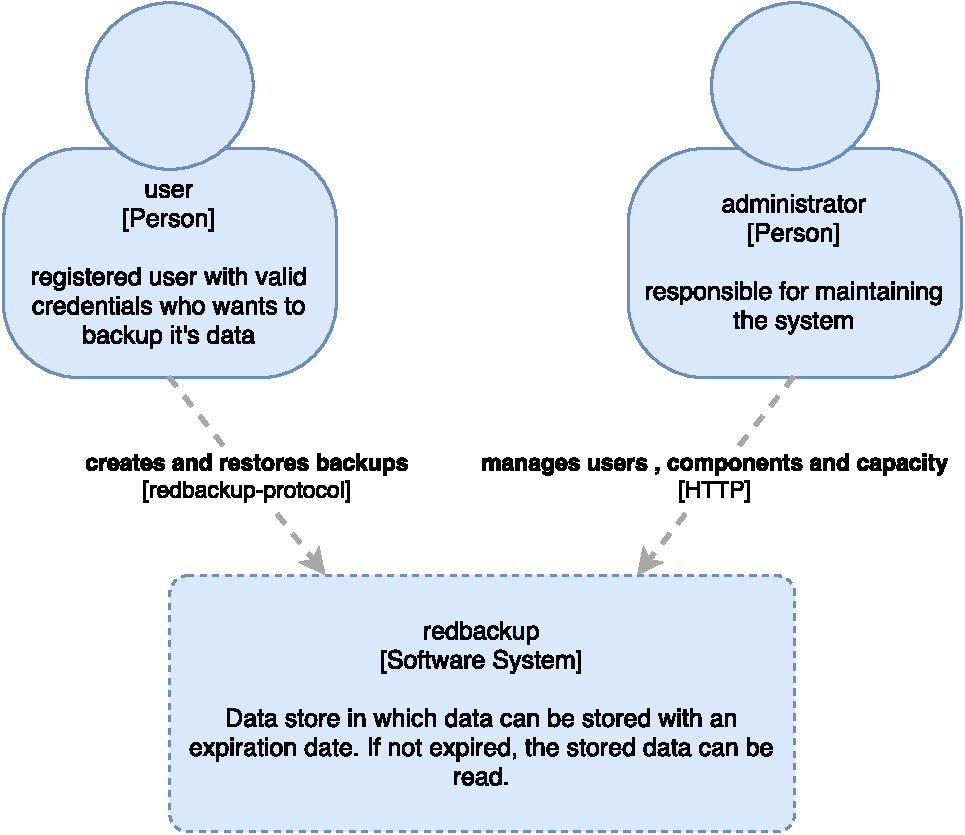
\includegraphics[width=0.8\linewidth]{resources/c4-overview}
	\caption[C4 System Context Diagram]{C4 System Context diagram showing the big picture.}
	\label{fig:c4-overview}
\end{figure}

Distinctive of both actors is that they do not want to interact directly with the system unless human interaction is inevitable. This takes the burden of manually creating backups away from the user including the risk of oblivion and minimises management efforts required by the administrator.  

Both actors, as well as their intentions, are described in more detail in Appendix \fullref{sec:specification}. Figure \ref{fig:c4-overview} presents a high-level overview that illustrates the interactions of the actors with the redbackup system.

\paragraph{Structure}
The redbackup system consists of four core components as shown in the C4 Container diagram in Figure \ref{fig:c4-container}.

\begin{figure}[h]
	\centering
	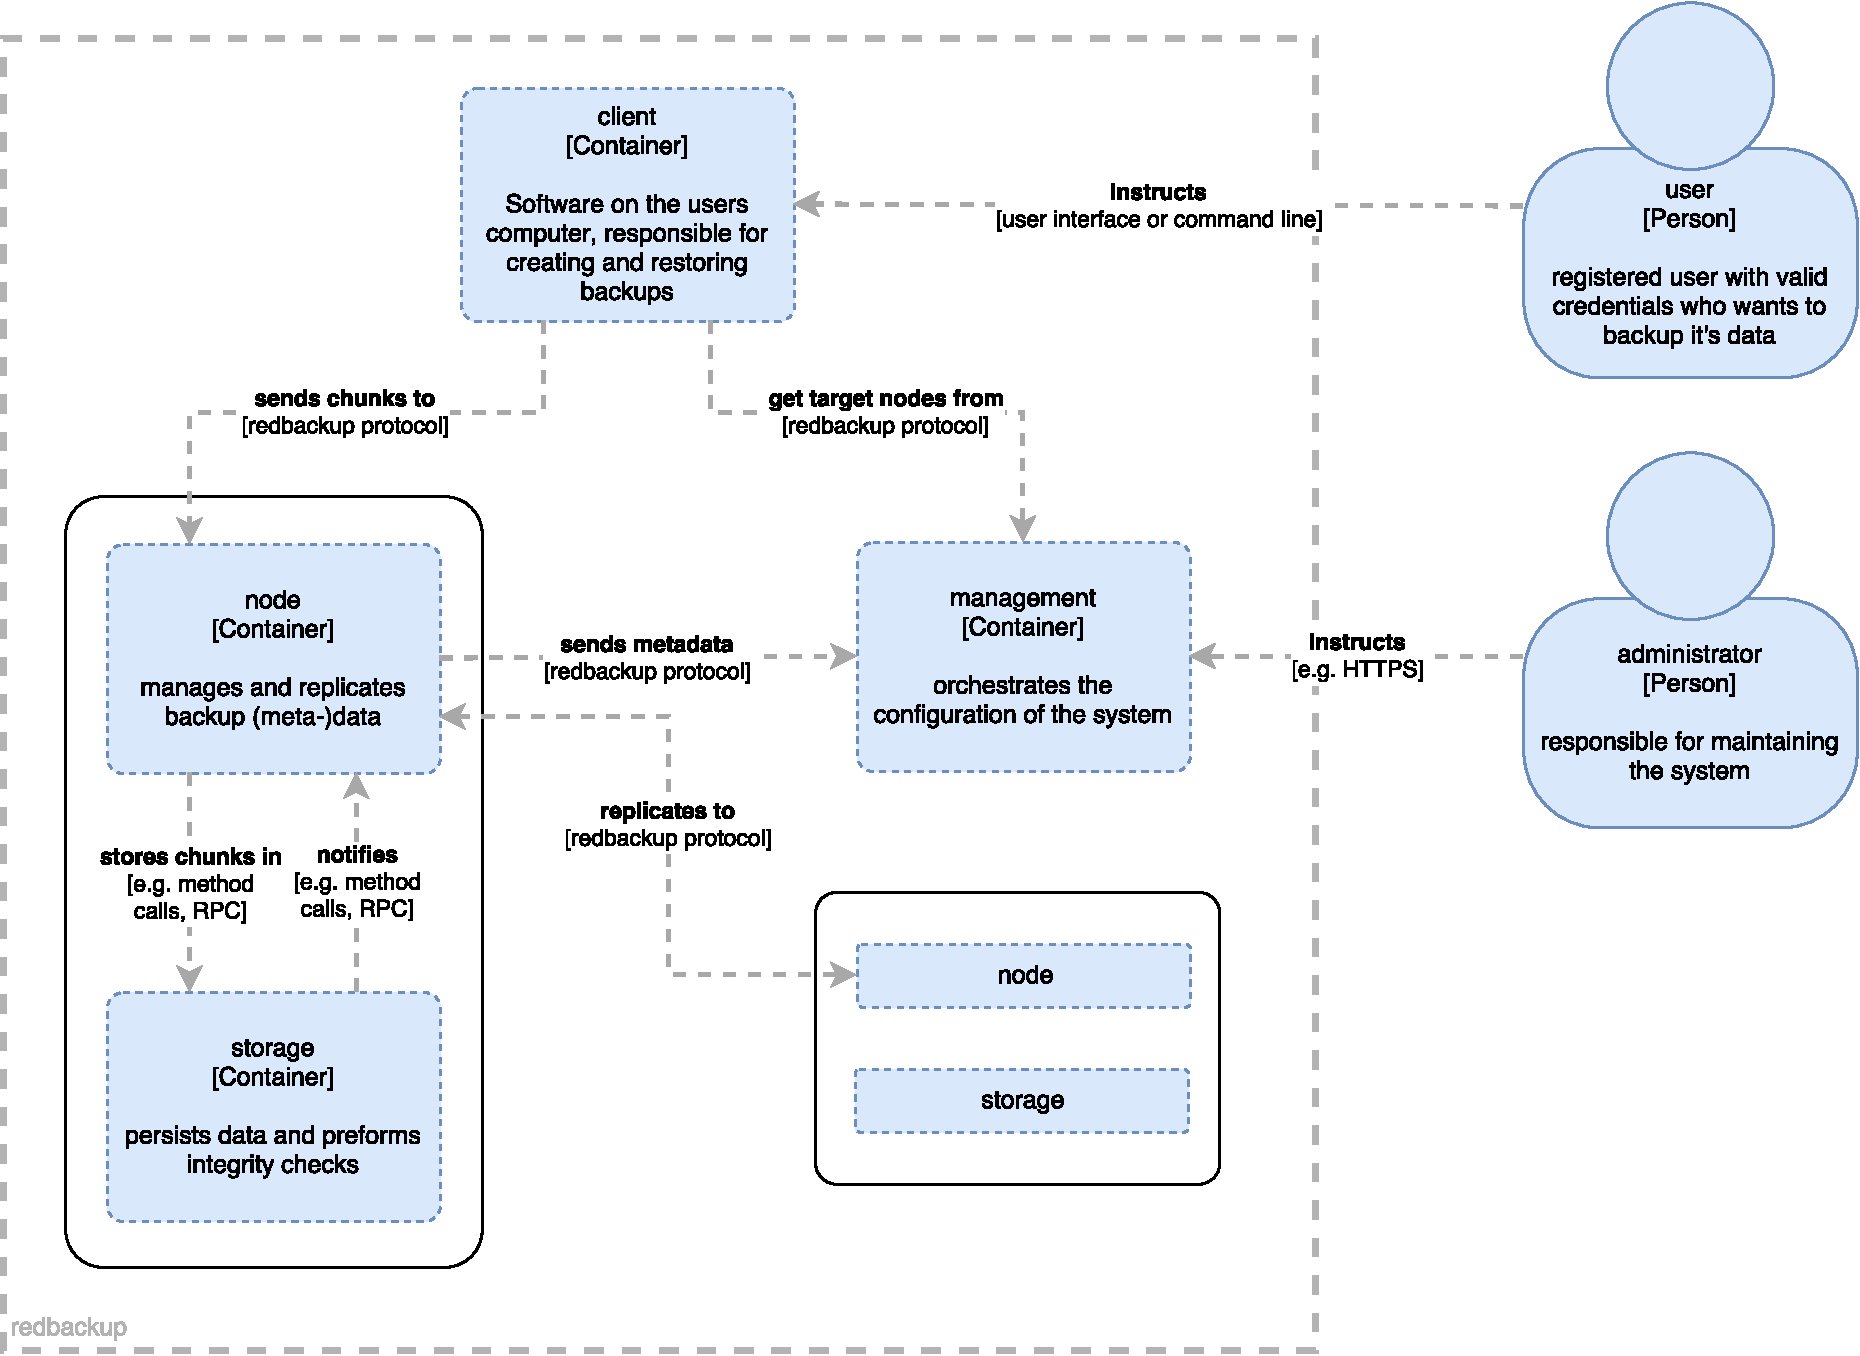
\includegraphics[width=1\linewidth]{resources/c4-container}
	\caption[C4 Container Diagram]{C4 Container diagram illustrating the high-level shape of the redbackup software system and how responsibilities are distributed.}
	\label{fig:c4-container}
\end{figure}

\paragraph{Client} A \gls{user} instructs a \gls{client} program typically running on the users machine to perform (unattended) backups and restores.  A \gls{client} persists and loads its data from one or more interconnected \glspl{node}.

\paragraph{Node}
A \gls{node} is in charge of data \glspl{chunk} including their replication onto other \glspl{node}. \Glspl{node} persist the actual data in a separate component, a \gls{storage}, to encapsulate persistence from replication and interaction to support different kinds of storage technologies (e.g. plain file systems or databases). A \gls{node} and its \gls{storage} are typically deployed on the same host.

\paragraph{Management}
One central \gls{management} component orchestrates the configuration of the system by providing metadata to \glspl{client} and \glspl{node}. This metadata includes user information and a set of all \glspl{node} in the system including their addresses and states. \Glspl{client} and \glspl{node} must cache this metadata which ensures that a temporary unavailability of the \gls{management} component does not compromise the replication and backup process.

All components including their responsibilities and interactions are described in more detail in Appendix \fullref{sec:specification}.

\paragraph{Protocols} Redbackup specifies a high-level protocol that is used for internal communication (noted in all C4 diagrams as \emph{redbackup protocol}). We deliberately specified the communication on a high level to encapsulate the underlying transport mechanisms.

\subsection{Backup creation}
\begin{figure}[h]
    \centering
    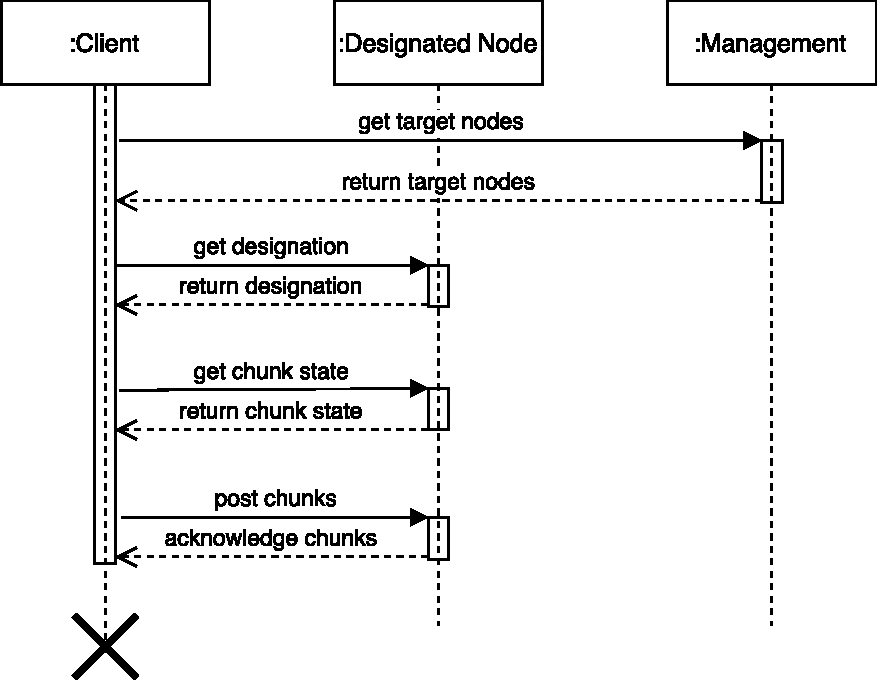
\includegraphics[width=\linewidth]{resources/create_backup_designated}
    \caption[Create Backup UML Sequence Diagram]{UML sequence diagram illustrating the communication during the creation of a backup.}
\end{figure}

To create a backup, a \gls{client} loads all \gls{node}-metadata, that includes the addresses, from the \gls{management}. The \gls{client} caches this set and chooses one of them as \gls{designated-node}. This selection can either be random or based on heuristics, e.g. by analysing the round trip time to a \gls{node}.

The \gls{client} then requests permission to perform a backup on a given \gls{designated-node} by sending a \emph{get designation} message that includes an estimated backup size and the \gls{expiration-date}. If the \gls{designated-node} has the storage capacity as well as other resources available (i.e. it is not under overload), it confirms the designation request.

By now, the \gls{client} must start to build up backup metadata - hereafter called \gls{chunk-index} - by walking recursively through all directories to backup. Each file that is not explicitly excluded is split up into one or more data \glspl{chunk} using a rolling hash\cite{borg-data-structures}. Each of these \glspl{chunk} are then encrypted individually. Afterwards the \gls{client} derives the identifier of every \gls{chunk} based on its contents. This mechanism enables deduplication. Section \fullref{sec:fundamental-design-decisions} discusses \glspl{chunk} and \glspl{chunk-identifier} in detail.

The \gls{client} sends the calculated \glspl{chunk-identifier} at regular intervals to the \gls{designated-node}. The \gls{designated-node} returns a subset of all \glspl{chunk-identifier} of the \glspl{chunk} that are already present on it.

The \gls{client} then posts the missing \glspl{chunk} to the \gls{designated-node} which acknowledges successful receipt.

When all \glspl{chunk} are transmitted successfully, the client encrypts the \gls{chunk-index} as well and sends it to the \gls{designated-node} using the same mechanism as for any other \gls{chunk}. The only difference is that an additional flag - hereafter called \gls{root-handle} - is set so that it can be found again for restore.

The detailed backup scenario can be found in Appendix \fullref{sec:scenario-create-backup}.

\subsection{Backup restore}

\begin{figure}[h]
    \centering
    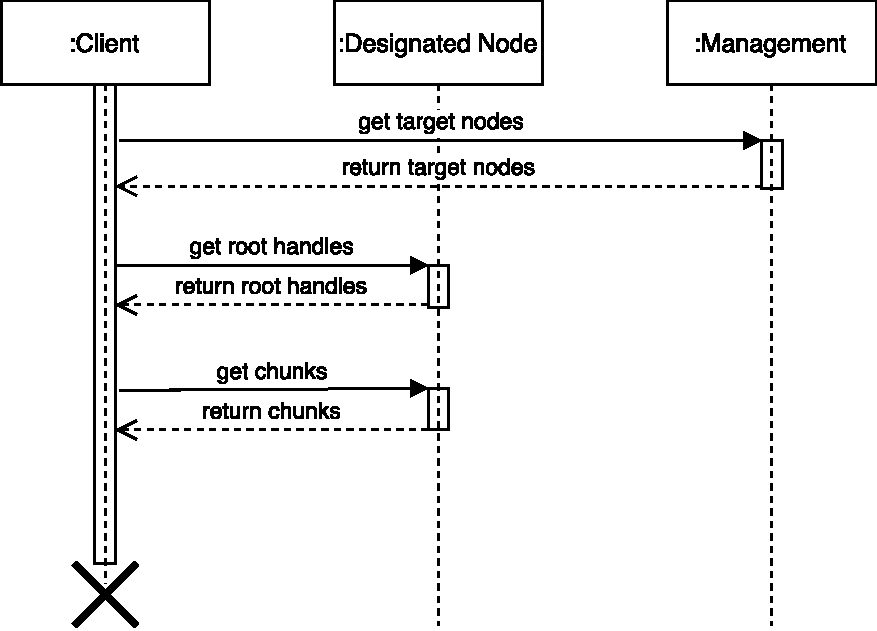
\includegraphics[width=\linewidth]{resources/backup_restore_designated}
    \caption[Backup Restore UML Sequence Diagram]{UML sequence diagram illustrating the communication during the restore of a backup.}
\end{figure}

The restore mechanism works identical to the backup process up to the point where a \gls{designated-node} is chosen.

Next, the \gls{client} loads all \glspl{root-handle} from the \gls{designated-node}. The \gls{client} can decrypt the \glspl{chunk-table} from the returned \glspl{chunk-content}. Based on this information, the \gls{client} can provide multiple restore options to the \gls{user}, e.g. to restore a particular version of a given file.
With the user input and the previously fetched \glspl{chunk-table}, the \glspl{client} can calculate which \glspl{chunk} must be requested from the \gls{designated-node}. \Glspl{chunk-content} are then downloaded at regular intervals from the \gls{designated-node}, decrypted and combined.

\subsection{Replication}\label{sec:replication}
% Planned and unplanned leaving of nodes
% Management down
We deliberately only specified \gls{system-n-replication}, which means the degree of redundancy for the entire system is equal to the amount of \glspl{node} in the system (see \fullref{sec:fundamental-design-decisions}).

A \gls{node} is in charge of all data stored on it. Each \gls{node} - hereafter called \gls{sending-node} - randomly picks $n$ of its data \glspl{chunk}. It then picks one other \gls{node} randomly - hereafter called \gls{designated-node} - and requests which of the chosen data \glspl{chunk} remain persisted on the \gls{designated-node}. The \gls{designated-node} returns a subset of the requested \glspl{chunk} that consists of all \glspl{chunk} that it owns. Using this response, the \gls{sending-node} sends all missing \glspl{chunk} to the \gls{designated-node} which acknowledges successful receipt.

\begin{figure}[h]
    \centering
    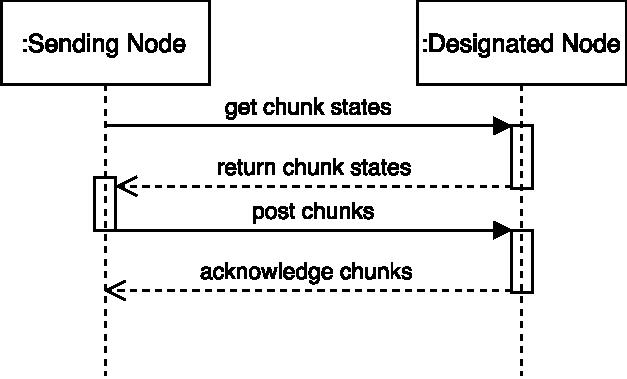
\includegraphics[width=0.6\linewidth]{resources/data_replication_designation}
    \caption[Data Replication UML Sequence Diagram]{UML sequence diagram illustrating the communication during replication.}
\end{figure}

This scenario is described in more detail in the Appendix \fullref{sec:scenario-data-replication}.

\subsection{Security and Encryption}\label{sec:security-and-encryption}
\paragraph{Data Integrity} One of our primary design goals is to ensure that once data is in the redbackup system, it cannot be altered or deleted from a \gls{client} to prevent ransomware attacks \cite{young-cryptovirology}. To achieve this, each backup is provided with an \gls{expiration-date} on which \glspl{node} are allowed to remove the associated data. 

Reasoning and potential risks of physical time are discussed in section \fullref{sec:removal-of-old-backups}.

\paragraph{Data Integrity on Nodes} Because \glspl{node} can also be the target of randsomware attacks, each \gls{node}, or more precisely its associated \gls{storage} component, must verify that given \glspl{chunk-content} are not corrupted. To be able to do so, it must be possible to calculate the identifier of such a data \gls{chunk} from its contents, using cryptographic hash functions.

A discussion on the role of hash functions including the chosen algorithms for the study project is carried out in section \fullref{sec:hash-collisions}.

\paragraph{Data Integrity on the Management} The \gls{management} component has no knowledge of the persisted data in the system. It only manages configuration and must not have detailed knowledge of \glspl{chunk} (need-to-know principle \cite{security-patterns}).

\paragraph{Data Encryption} A \gls{client} encrypts \glspl{chunk} when creating a new backup. This ensures that no other participant in the redbackup system can inspect file contents (need-to-know principle \cite{security-patterns}). The encryption and decryption keys are only stored on the \gls{client} and must be backed up separately.

\paragraph{Transport Security} All sent \glspl{message} should be signed by the sender. If so, transport layer encryption is not strictly necessary because all user data is already encrypted on the \gls{client} with the only exception of the \gls{expiration-date}.
\\
\vspace{1em}

\noindent A detailed description of these security mechanisms would be out of scope for this study project and will have to be carried out in a next step.

\subsection{Partitioning \& Scaling}

\paragraph{Availability \& Overload} To scale the redbackup system regarding availability, more \glspl{node} can be added to the redbackup system. If a given \gls{node} is overloaded, a \gls{client} can use another \gls{node} for backup creation or restore.

Because the backup and restore processes require approval of a \gls{designated-node} (see scenarios \fullref{sec:scenario-create-backup} and \fullref{sec:scenario-backup-restore}), an overloaded \gls{node} can finish work in progress backups/restores and reject new requests (following the patterns Finish Work In Progress and Shed Load \cite{fault-tolerance}). The data is replicated to overloaded \glspl{node} eventually.

We ensured that \glspl{node} are (mostly) stateless which simplifies scaling as well.

\paragraph{Storage Scalability} Because the proposed system currently only supports \gls{system-n-replication} (see section \fullref{sec:fundamental-design-decisions}), the maximum storage capacity is equal to that of the \gls{node} with the smallest storage. Therefore, to increase storage capacity, the capacity of all \glspl{node} must be extended to meet the desired amount.

To minimise network usage deduplication of data is used on the \gls{client}. Deduplication is  discussed in the paragraph Storage Unit in  \fullref{sec:fundamental-design-decisions}.

\subsection{Failure Detection}

Additionally to the above-discussed mechanisms for fault tolerance regarding security and scaling, the following failure detection mechanisms are in place.

\paragraph{Reporting} Most issues that occur on a \gls{node} are reported to the \gls{management} component (following the pattern Someone in Charge \cite{fault-tolerance}). The \gls{management} can then decide to notify the system administrator or execute error mitigation processes, e.g. suspend a given \gls{node} temporarily.

If a \gls{node} tries to connect to another \gls{node} that is not available, it notifies the \gls{management} component (following the pattern System Monitor\cite{fault-tolerance}).

Each \gls{node} periodically checks the persisted contents for possible corruption using the checksum mechanisms discussed in \fullref{sec:security-and-encryption} (following the Pattern Routine Audits \cite{fault-tolerance}). If a corruption is detected, the \gls{storage} notifies the \gls{node} which notifies the \gls{management}.

\paragraph{Single Point of Failure} For the case that the \gls{management} component is temporarily unavailable, \glspl{node} and \glspl{client} cache metadata, e.g. information about other \glspl{node}. Using these caches, \glspl{node} can perform replication and \glspl{client} manage their backups without interruption. Any notifications that were not successfully transmitted to the \gls{management} must be buffered on the \glspl{node} in order to ensure their delivery.

\section{Fundamental Design Decisions}\label{sec:fundamental-design-decisions}

We used the morphological box technique to explore different possible implementation options (see Table \ref{tbl:morphological-box}). The chosen option should be as simple as possible for the prototype developed in the study project but extensible for further adaption.

The following paragraphs reason the selected entry in each dimension.

\paragraph{Redundancy}

We originally planned to support \gls{client-m-replication}, which means that the \gls{client} defines a custom degree of redundancy from 1 to the number of \glspl{node} in the system. However, this is a complex mechanism that requires sophisticated algorithms to work correctly and efficiently. For the prototype, we chose the more straightforward implementation option system \gls{system-n-replication}, where the degree of redundancy for the entire system is equal to the number of \glspl{node} in it. Changing this option in the future will not be trivial because it requires additional changes in the replication process and the communication protocols.

\paragraph{Storage Unit}
The idea of \emph{chunks} come from Borg Backup. Files are partitioned into chunks using a rolling hash which enables deduplication and space efficient backups for large files \cite{borg-data-structures}. These are desired properties in a backup system to minimise network and disk usage.

\emph{Encrypting chunks} means that deduplication of the same file coming from different users is not possible anymore but is a necessity for privacy. Encryption is not trivial and requires a user concept that is out of scope of the prototype developed in the study project.
We chose the \emph{plain files} option for the study project to simplify the \gls{client} implementation. In the future, supporting \emph{encrypted chunks} will be possible by just modifying the \gls{client}.

\paragraph{Role of the Management}
The \emph{one in charge} option is the most straightforward option to implement, but conflicts with many intentions of the administrator (see \fullref{sec:adminstrator-intention}). We also intended to avoid a single point of failure. We chose the option \emph{autonomous replication} because it guarantees that replication is always ensured and keeps communication relatively simple.

\paragraph{Storage Backend}
Using the file system is the simplest possible solution for the study project and therefore the selected option. Adding support for other backends in the future is still possible because the storage component is an isolated part in the architecture (see \fullref{sec:component-storage}).

The number of files in a folder is limited depending on the used file system, length of a filename and other factors. Some file systems (e.g. ext4) have a global limit for the maximal number of files. This limit is 4 billion files for ext4. \cite{ext4}. Therefore we use the ext4 file system to persist data in the study project.

\paragraph{Removal of Old Backups}\label{sec:removal-of-old-backups}
We decided to use \emph{physical time}stamps that must be specified on backup creation. After expiration, the backup data may be removed by a garbage collector running on a \gls{node}. This may be extended to allow only mutual garbage removal in the future.

A significant problem that \emph{physical time} addresses is the safety of backup data in case a user computer is infected with malware~\cite{young-cryptovirology}. An illicit application might command the removal of backups or create new backups to initiate a garbage collection process to free storage capacity.

Nevertheless, the use of \emph{physical time} has the downside of possible data loss in case of wrong system times. To mitigate this risk, the system should use multiple distinct upstream time-servers. Multiple distinct upstream time-servers are used with a high probability as the proposed redundancy model motivates users to expand the system across multiple physical locations. Furthermore, the \gls{client}, \glspl{node} and \gls{management} should verify a reasonable accurate time when communicating mutually.

\paragraph{Programming Language \& Ecosystem}
We chose Rust over Erlang and Go because it offers great performance and minimal overhead supported by a powerful type system.
A complete language evaluation can be found in \fullref{sec:language-evaluation}.

\begin{sidewaystable}
	\centering
	\caption[Morphological Box]{Morphological Box}
	\label{tbl:morphological-box}
    \begin{tabu}{X | X X X X}
		\hline
          \textbf{Redundancy}
          & No redundancy
          & \Gls{client-m-replication}: The \gls{client} defines a custom degree of redundancy (from 1 to the number of \glspl{node}).
          & \Gls{system-m-replication}: The administrator defines the degree of redundancy for the entire system (from 1 to the number of \glspl{node}).
          & \textbf{\Gls{system-n-replication}}: The degree of redundancy for the entire system is equal to the amount of \glspl{node} in the system.
          \\ \hline

          \textbf{Storage unit}
          & \textbf{Plain files}
          & Encrypted files
          & Chunks: Cut files into multiple parts and store these individually.
          & Encrypted chunks: Same as chunks, but every chunk is individually encrypted.
          \\ \hline


          \textbf{Role of the management}
          & One in charge: The management knows and controls everything (e.g. the location of every file/chunk).
          & Configuration only: The management must be available for administrative tasks only. The \glspl{node} are mostly autonomous.
          & \textbf{Autonomous replication}: The management must be available for most of the tasks but replication also works if the management is down.
          & No management: Every \gls{node} is completely autonomous.
          \\ \hline


          \textbf{Storage backend}
          & \textbf{Plain filesystem}: Store all files/chunks as files in one directory with a unique identifier.
          & Database: Use an existing database solution (e.g. Git, Redis, RocksDB).
          & Cloud Storage: A proxy to a cloud storage provider (e.g. Amazon S3).
          & Custom: An optimized version of the plain file system option with optimised indexing and compression.
          \\ \hline


          \textbf{Removal of old backups}
          & \textbf{Physical time}: Data is removed on a specified physical time.
          & User command: The user commands removal of data.
          & Free storage: Data is removed, as soon as capacity issues occur.
          & Physical time with mutual agreement: All \glspl{node} must agree before data is removed.
          \\ \hline


          \textbf{Programming language / ecosystem}
          & \textbf{Rust}
          & Go
          & Erlang
          & 
          \\ \hline
	\end{tabu}
\end{sidewaystable}

\subsection{Hash Collisions}\label{sec:hash-collisions}
To achieve deduplication and space-efficient backups for large files, as discussed above, a chunk identifier must be derived from the actual chunk contents. 
A common mechanism used to derive identifiers from binary data is the use of cryptographic hash functions. Most cryptographic hash functions produce a message digest that has a fixed length (e.g. SHA-256\cite{sha-256} produces a 256-bit digest) for a given message with an arbitrary length. The restricted length can theoretically lead to collisions.
Perfect hash functions do not have this property because their input message length is equal to the length of the resulting message digest. A perfect hash function is not practical in our case due to the large message digests.
With cryptographic hash functions, collisions are possible but unlikely. Assuming that the applied function does produce equally distributed results, the probability can be calculated based on the birthday problem\cite{birthday-attack} as follows, where $p$ is the number of chunks in the system and $n$ the length of the message digests:

\[
P(p, n) = \frac{p^2}{2^{n+1}}
\]

Assuming we have $p=30^{21}$ chunks the system (which is equivalent to two billion years of music assuming each chunk has a size of one byte\cite{seagate-zetabyte}) and using the SHA-256 algorithm, the probability of a collision is about $4.72 \cdot 10^{-16}$, which is highly improbable and may therefore be neglected.

However, did a collision occur after all, for example, if the used cryptographic hash function were flawed or the unlikely event occurred, it would result in data loss.

In theory, we could detect collisions on the \gls{client}. To do so, every time an identifier is calculated, the \gls{client} must verify that if a chunk with the same identifier already exists in the system, it has the exact same contents. If the contents differ, it is a collision. This approach requires a lot of network traffic and can slow down the backup process significantly.

Another place to detect collisions is on the \gls{node} component. A \gls{node} can verify if the contents of a given chunk are equal to the contents already present in the system. The downside of this approach is that it requires the \gls{client} always to send the full contents of every chunk, which leads to a lot of additional network traffic.

Both of the described approaches for collision detection have significant costs that are not practical.

As for the study project, we use the SHA-256 algorithm\cite{sha-256} and neglect the risk of hash collisions due to its low probability. Nonetheless, we prepare all protocols and components to use an interchangeable mechanism for the calculation and transmission of file/chunk identifiers.

\section{Prototype}\label{sec:prototype}

Because the entire system, as described in the previous sections, is too large and complex to implement in the form of a study project prototype, we reduced the functionality to its core.

Our prototype focuses on the backup, restore and replication scenarios as described in Appendix \fullref{sec:scenarios} leaving out encryption.

We also limited the supported platforms to 64-Linux only as this is the operating system we use for development and continuous integration.

The implemented prototype is organised in 46 modules, defines 188 functions and has 4'240 lines of code, including unit test code and whitespace. All components are implemented using the Rust programming language \cite{rustlang-org}. Installation instructions are documented in the project's repository.

\subsection{Concrete Architecture}

Figure \ref{fig:c4-sa-container} illustrates the system as implemented in our prototype.

\begin{figure}[h]
	\centering
	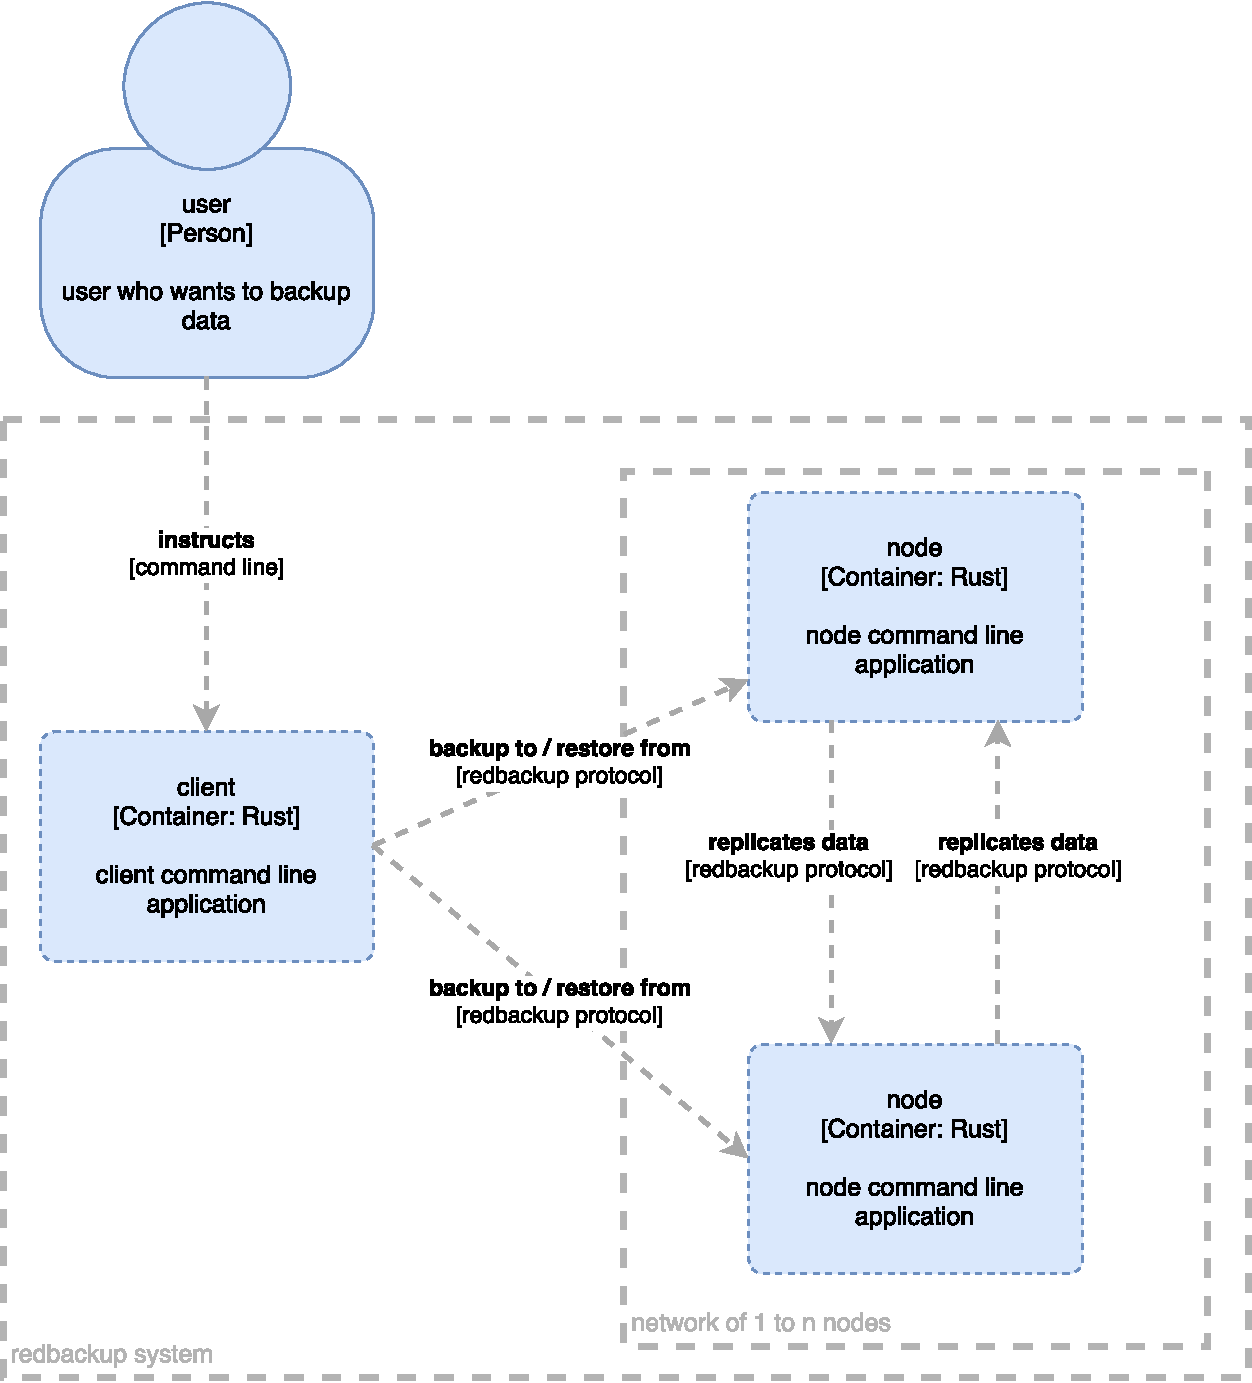
\includegraphics[width=0.8\linewidth]{resources/c4-sa-container}
	\caption[Study Project specific C4 Container Diagram]{C4 Container diagram illustrating the high-level shape of the prototype and how responsibilities are distributed as implemented in the study project.}
	\label{fig:c4-sa-container}
\end{figure}

The \gls{client} and \gls{node} are delivered as executables that are configured and launched using the command line.

The \gls{node} component binds itself to a configured network interface and port on which it provides the services for backup creation, backup restore and replication.

The \gls{client} executable is started individually for every operation that is the creation of a backup, listing all backups persisted on a given \gls{node} and data restore.

\subsubsection{Client}

The \gls{client} executable bundles three components as shown in Figure \ref{fig:c4-client-container}.

\begin{figure}[h]
	\centering
	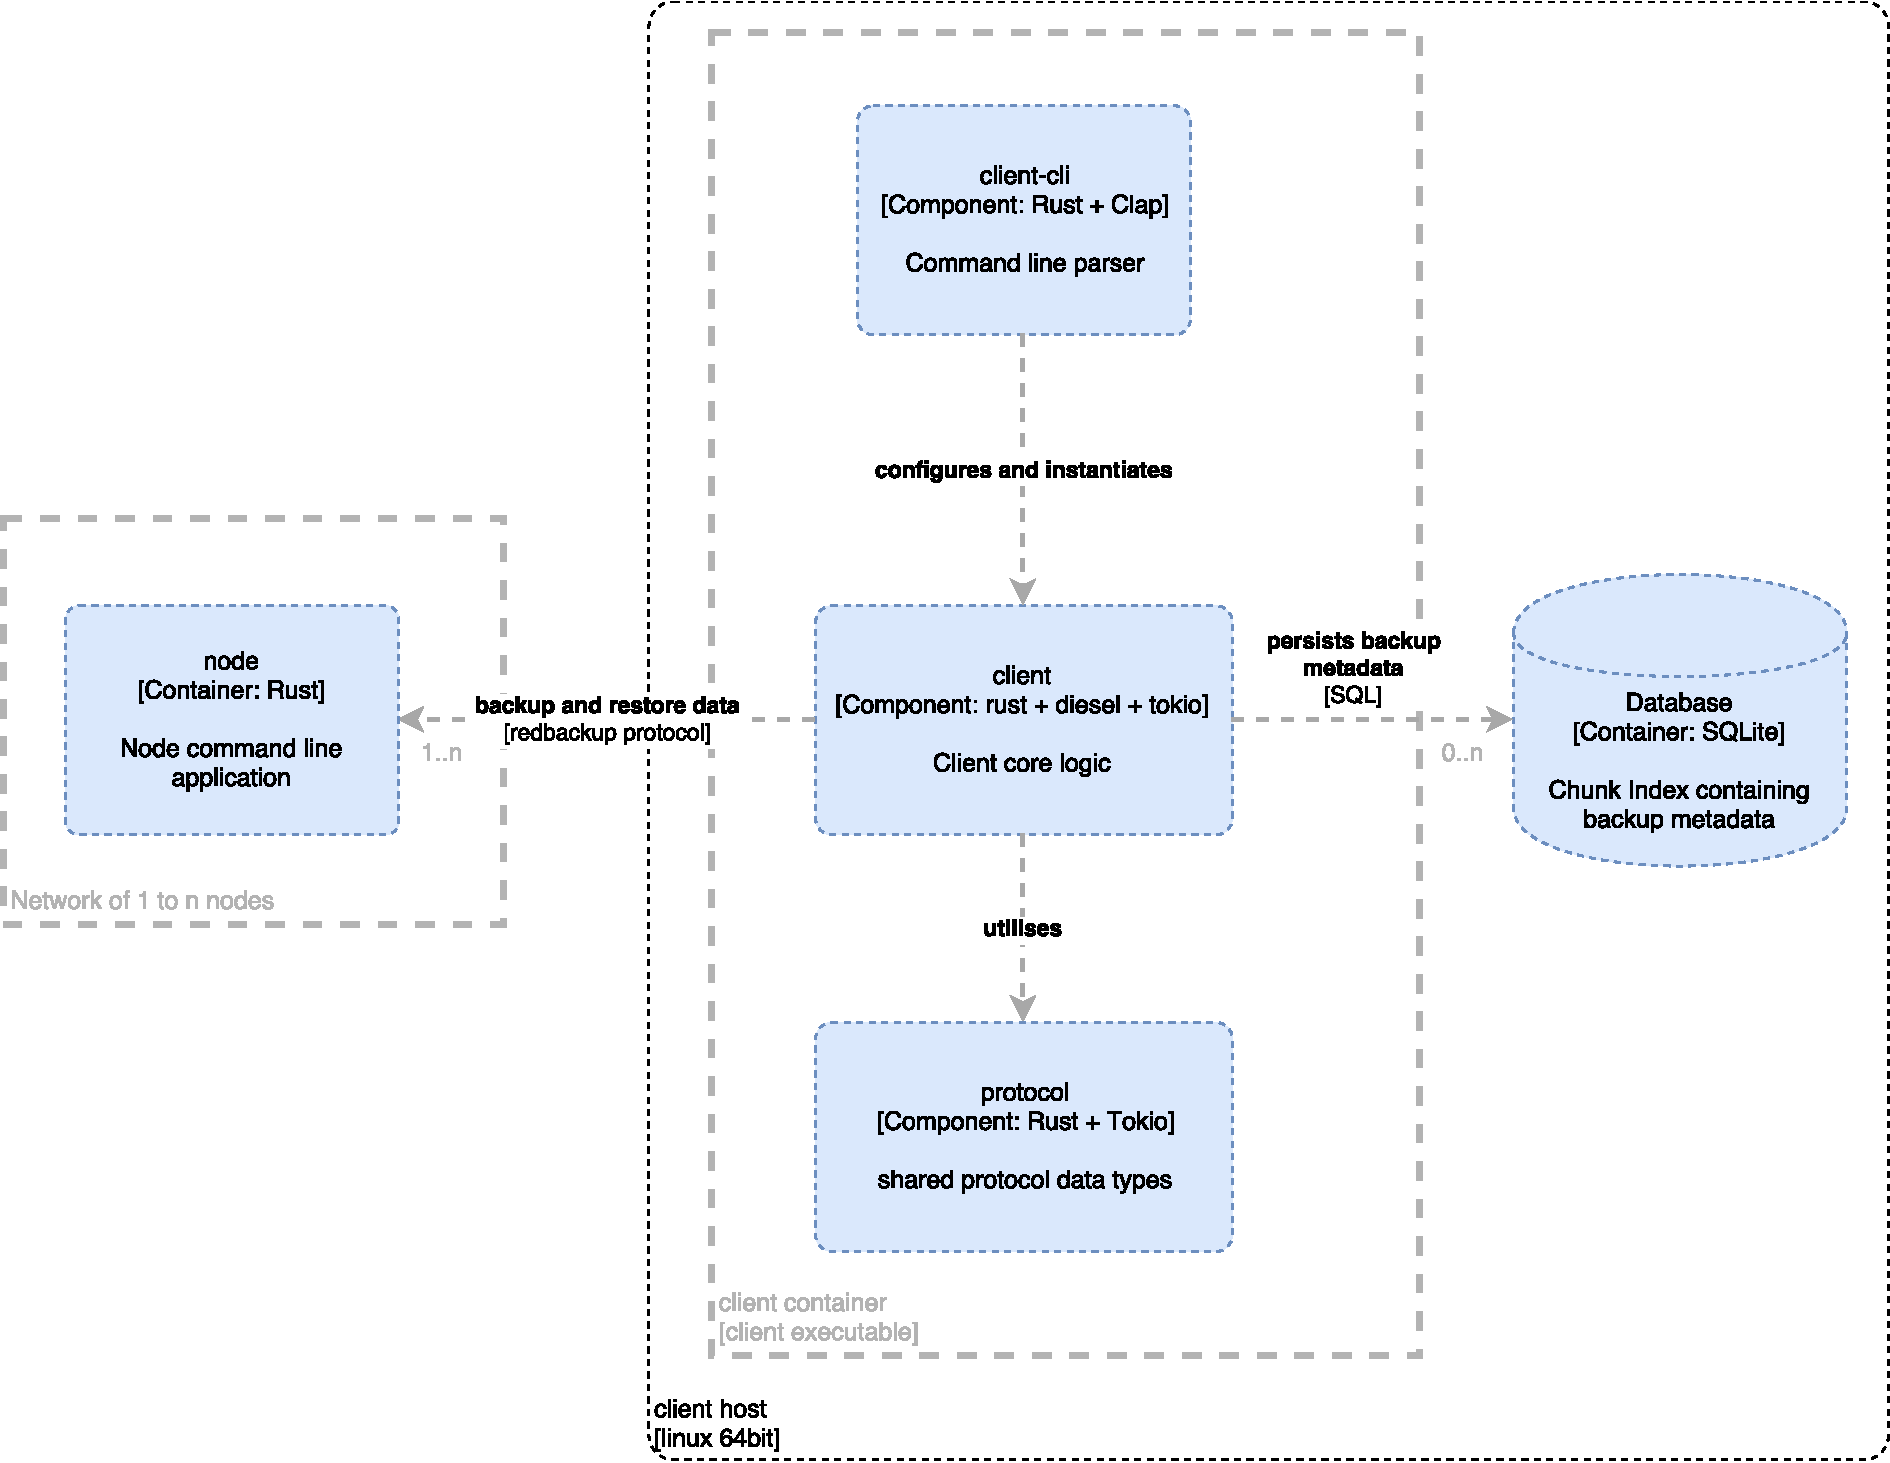
\includegraphics[width=1\linewidth]{resources/c4-client-container}
	\caption[Client specific C4 Container Diagram]{C4 Container diagram illustrating the shape of the \gls{client} and how responsibilities are distributed as implemented in the study project.}
	\label{fig:c4-client-container}
\end{figure}

\emph{Client-cli} contains the command line specific logic that provides an uncluttered interface for advanced users and serves as an entry point in the client's core logic. We used the clap\footnote{\url{https://clap.rs/}} library to implement this component. The command line interface is described in Appendix~\ref{sec:prototype-command-line-interface}.

The \emph{client} component contains the actual logic for creating and restoring backups. It is organised as a library so that it can be used from other projects as well, e.g. if we provide a graphical user interface in the future. The \gls{client} component creates the \gls{chunk-index} for every backup in a separate \emph{SQlite-database}. For database access, we used the Diesel\footnote{\url{https://diesel.rs/}} ORM-library.

The \gls{client} component makes heavy use of a networking library called tokio\cite{tokio-rs} that provides an efficient event loop similar to the Reactor pattern \cite{POSA1}. Although tokio supports highly parallel networking code, we decided to implement all interactions on the \gls{client} serial to maintain readability.

The (de-) serialisation mechanisms for messages sent to and received from \glspl{node} are encapsulated in the \emph{protocol} component, following the Forwarder Receiver Pattern \cite{POSA1}.

We opted for Diesel and tokio because there are currently no comparable alternatives on the marked in both application areas.

In the prototype, the \gls{client} interacts with one \gls{node} at a time to maintain simplicity. The \gls{node} to interact with is passed to the \gls{client} executable via command line arguments.

\subsubsection{Node}

The \gls{node} executable bundles four components as shown in Figure \ref{fig:c4-node-container}.  

\begin{figure}[h]
	\centering
	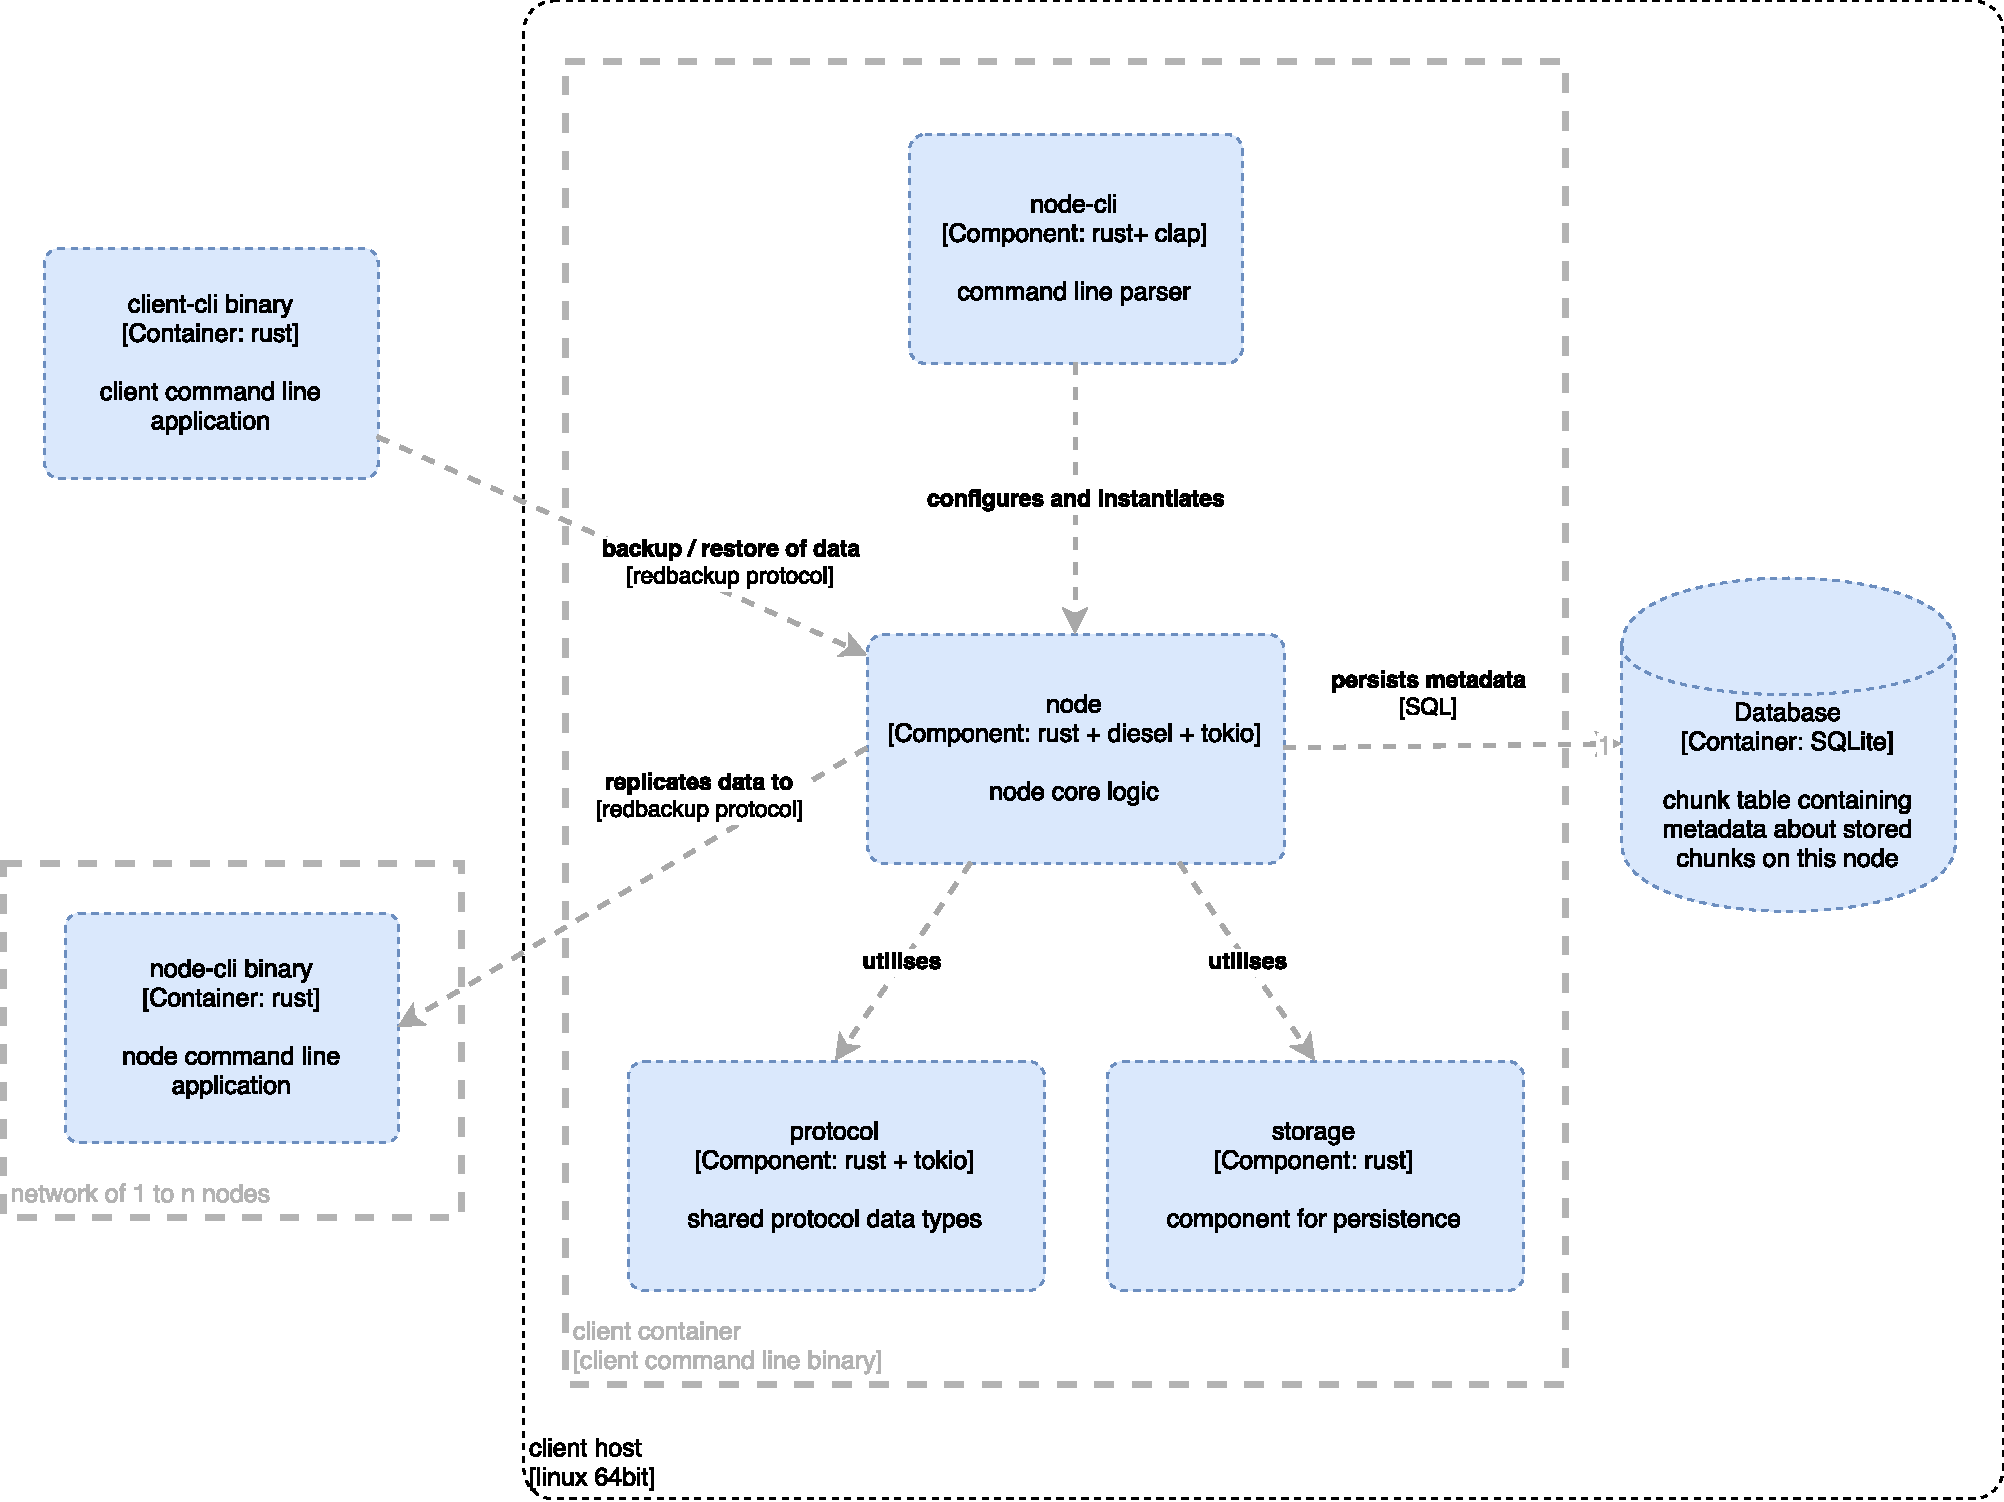
\includegraphics[width=1\linewidth]{resources/c4-node-container}
	\caption[Node specific C4 Container Diagram]{C4 Container diagram illustrating the shape of the \gls{node} and how responsibilities are distributed as implemented in the study project.}
	\label{fig:c4-node-container}
\end{figure}

Just like the \gls{client} implementation, the command line logic is encapsulated in a separate component called \emph{node-cli}.

The core logic is implemented in the \emph{node} library. Like the \gls{client}, the \gls{node} component makes heavy use of the tokio and Diesel libraries. In contrast to the client, we used the parallel features of tokio. To keep the chosen technology close to the client, we decided to use SQLite for the \gls{chunk-table}. This must be changed in the future because SQLite locks the entire database when writing, which makes concurrent updates impossible \cite{sqlite-locking}.

We use the same \emph{protocol} component for (de-) serialisation of messages on the \gls{node} and the \gls{client}.

The \emph{storage} component is also bundled directly in the \gls{node} executable. It persists data in one single directory as described in \fullref{sec:fundamental-design-decisions}.

Other known \glspl{node} are passed to the \gls{node} executable via command line arguments.

Because user authentication requires additional cryptographic efforts, the prototype accepts backups and replications from everyone.

\subsection{Testing}\label{testing}

In the following subsections, we describe how the prototype and architecture can be tested.

\subsubsection{Unit Tests}\label{unit-tests}
Test Driven Development (TDD) \cite{TDD} should be used as much as possible. Our Definition of Done (Appendix \ref{sec:project-plan}) states that \emph{reasonable unit and integration tests [must] exist and pass.}

All unit tests are executed on every build run on our continuous integration server. That is on every repository push and pull request.

\subsubsection{Integration Tests}\label{integration-tests}

We defined two primary environments for the integration tests: A minimal network as defined in Figure \ref{fig:integrationtestsmall} and a medium one, as defined in Figure \ref{fig:integrationtestmedium}.

\begin{figure}
	\centering
	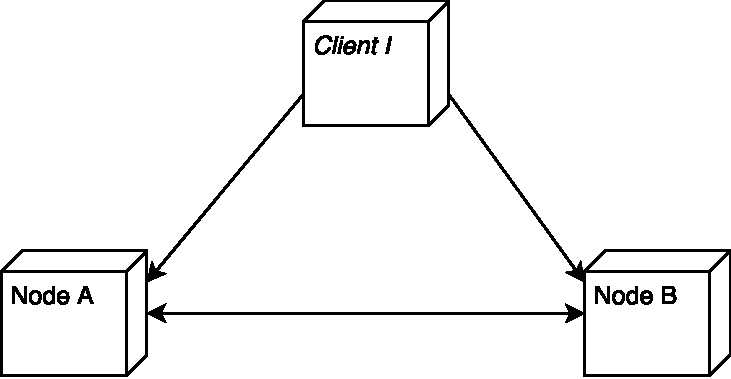
\includegraphics[width=0.5\linewidth]{resources/integration_test_small}
	\caption[Minimal integration test]{Minimal integration test with one \gls{client} and two \glspl{node}.}
	\label{fig:integrationtestsmall}
\end{figure}

\begin{figure}
	\centering
	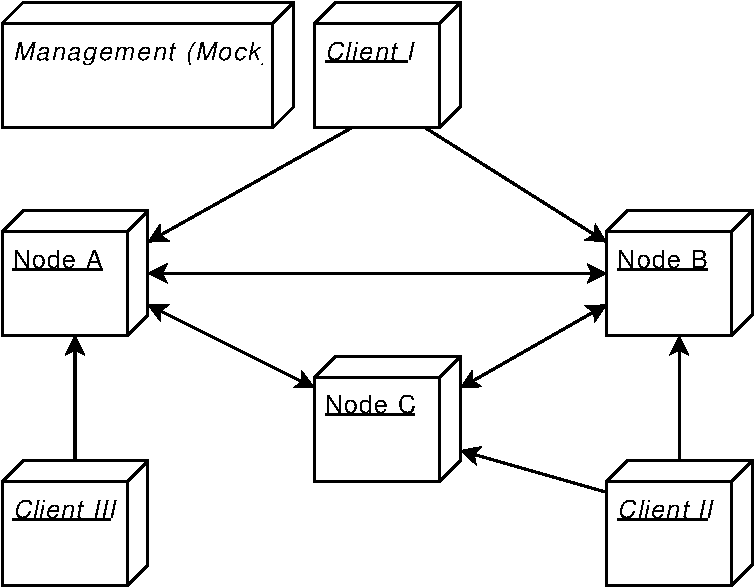
\includegraphics[width=0.5\linewidth]{resources/integration_test_medium}
	\caption[Medium integration test]{Medium integration test with three \glspl{client} and three \glspl{node}.}
	\label{fig:integrationtestmedium}
\end{figure}

These two rather small network styles will most commonly be deployed, yet they can expose most of the possible problems.

The integration tests are run automatically at least on every tagged release (i.e. at least once every sprint). Because of the (yet) well manageable set of integration tests for the prototype, these tests can run on every build as well.

Tests for fault tolerance, e.g. what happens if a \gls{node} goes down while receiving data, can be implemented as integration tests as well.

\subsubsection{Architecture tests}

Architectural tests are special and manually run tests to verify the scalability of our software architecture.

% !TeX spellcheck = en_GB
\chapter{Discussion and Conclusion}
\label{sec:discussion-and-conclusion}
This chapter contains our achieved results and lessons learned, discusses future work and closes with a conclusion.

\section{Achieved Result}

\subsection{Prototype}

In our prototype, we implemented the basic concepts of our architecture in a limited form. Rust was undoubtedly an excellent choice as a programming language for the prototype regarding robustness and performance but turned out to have a very steep learning curve. The same applies to the used frameworks tokio and Diesel. For this reason, we had to compromise to demonstrate as much of the architecture as possible without spending too much time on learning Rust.

Nevertheless, our implementation is solid and proves that the proposed architecture is robust and can be pursued further.

\subsection{Prototype Test Results}

\paragraph{Unit Tests}
We used test driven development (TDD) to develop the prototype as much as possible, which turned out to work great in the Rust ecosystem.

Some unit tests written for the prototype are not pure unit tests but minimal integration tests. Because Rust is not a traditional object-oriented language, it is not possible to introduce and use interfaces (Traits) in the same way as we were used to from other languages such as Java or C\#. Due to the steep learning curve Rust has, we were not able to fully utilise the corresponding mechanisms.

\paragraph{Integration Tests}

To write comprehensive black box integration tests, we created a testing library written in Python\footnote{\url{https://www.python.org/}}. In this framework, the internals on how to launch and configure \glspl{client} and \glspl{node} is encapsulated in classes. Using this abstraction, we decided to launch \glspl{client} and \glspl{node} in separate Docker\footnote{\url{https://www.docker.com/}} containers, so that they are as isolated as possible. All containers used in a test case are connected to a dedicated Docker network, which eliminates possible interferences with other network services.

We wrote integration tests that verify that a backup is flawlessly created, restored and replicated onto other \glspl{node}.

\paragraph{Test coverage}

Because Rust is still a young language with a relatively small ecosystem, tools for measuring code quality are still rare and immature. For our unit tests, we used Tarpaulin\footnote{\url{https://github.com/xd009642/tarpaulin}} to generate code coverage. Tarpaulin does not (yet) cover all language features and therefore returns a conservative coverage number. We achieved 53.5\% line coverage. This number would be significantly higher if all executed lines were counted correctly  (e.g. generated code using macros as well as compiler optimisations are not counted).

Code coverage achieved using the integration tests is not yet supported by any tool known to us and therefore undocumented. The integration tests do however cover all positive scenarios that were implemented.

Our integration testing framework allowed us to write such tests in a simple fashion.

\subsection{Architecture}

The architecture we elaborated in Chapter 2 and Appendix \ref{sec:specification} turned out to to be stable. It has proven advantageous that we did not specify too many details at the beginning (for example, the protocol) but focused on the high-level view.

\subsection{Architecture Test Results}

To ensure the validity of the proposed architecture, we manually ran architecture tests. We focused on scalability, data capacity and concurrent backups. We used our integration test framework for these tests as well.

\subsubsection{Overall Performance}\label{sec:overall-performance}

The conducted architecture tests on the prototype have shown a solid overall performance. Unfortunately, we observed significant memory consumption and CPU utilisation during most test scenarios.

\paragraph{CPU Utilisation}
Replication and the creation of a backup require a lot of CPU time on the \gls{node} and \gls{client} components. The \gls{client} components must execute many hash functions during the creation of chunks. A \gls{node} must verify that the provided chunk identifiers can be derived from the sent chunk contents during backup creation and replication.

Intensive CPU utilisation can be problematic, especially on a \gls{node}. This is somewhat an inherit problem of the propsed architecture because these calculation are required to ensure the integrity of the data stored in the system.

To mitigate this issue, a queuing mechanism can be implemented on the \gls{node} component that temporarly accepts chunks without performing integrity checks. These integrity checks can be performed in the near future and the sent chunks can afterwards be added definetly to the chunk table. The backup and replication protocol need to be adapted to signal this temporary queuing on a \gls{node} to \glspl{client} or other \glspl{node}. A new state (e.g. queuing) could be sent instead of an acknowledgement that instructs \glspl{client} and \glspl{node} to ask again for acknowledgement later.

It has to be investigated whether specific CPU acceleration for hash calculation could mitigate this problem as well.

\paragraph{Memory Concumption}
To prevent premature optimisation, which Donald Knuth famously pointed out is the root of all evil \cite{knuth-optimise}, we implemented \glspl{message} without streaming support. We implemented the high-level redbackup protocol as framed Message Pack\footnote{\url{https://msgpack.org/}} encoded \glspl{message} based directly on TCP. Such a Message Pack \gls{message} is (de-)serialised at once. In other words, whenever a \gls{message} is created or received, all its contents including the payload is loaded into memory. This decision, in combination with the design decision to not split up large files into multiple chunks, has led to significant memory consumption.

The protocol details must be clarified in the future to allow \gls{message} streaming. Refactoring the protocol component to use streaming mechanisms is feasible since Tokio provides these mechanisms\cite{tokio-streaming}. 

\subsubsection{Size Scalability Test Results}
As per our requirements in Appendix \ref{requirements}, the architecture should scale up to 100~\glspl{node}.

To test this scenario, we used the same underlying techniques as in our integration tests, but scaled the infrastructure up to 100 \glspl{node}.

Due to the high memory consumption, we were not able to conduct this test with a significant amount of data. A test run during which a 5MB file was replicated to 99 Nodes did not indicate a degraded performance.

\subsubsection{Data Capacity Test Results}
Our requirements (Appendix \ref{requirements}) also state, that a \gls{node} must be able to handle up to e.g. 2TB of data. To test this requirement, we planned to create large amounts of random data that has to be stored. This is a realistic requirement, as e.g. a compressed image, audio and movie collection might reach such sizes in practice.

It was not possible yet to create one single backup of 2TB at once due to the high memory consumption. Performing multiple backups in a row of a smaller dataset (i.e. 5 files with a size of 500MB) has not shown a decrease in performance.

\subsubsection{Concurrent Test Results}

We ran a test in which 5 \glspl{client} back up randomly generated data onto three randomly chosen \glspl{node}. On average, the entire backup process of 1MB data \gls{chunk} took 90-130ms from one docker container into another. These results clearly support our proposed architecture.

In reality, where \glspl{client} and \glspl{node} are on separate physical machines, this time will be significantly higher due to network latency. Also, because the creation of backups require a lot of CPU time, running all \glspl{client} on one machine is somewhat problematic. It is likely, that running all \glspl{client} and \glspl{node} on separate machines would improve the performance slightly.

\section{Lessons Learned}
% Describe what worked well and what went wrong (Lapses)
% What took us time?
% Summarize issues discussed in the retros

In this section, we describe unexpected project events and the lessons we learned from them.

\subsection{Project course}
\subsubsection{Documentation}
While discussing the documentation efforts in mini-retrospective two, we noted that some terms like metadata or chunks were not defined unambiguously and therefore used for different concepts in varying contexts. To standardise these, we decided to introduce a glossary that uniquely and precisely defines each of these terms.

While elaborating the architecture, we started researching advanced data distribution mechanisms and consensus algorithms. We were both very interested in these topics, but after a discussion with Prof.~Mehta and retrospective one, we realised that the time frame of the study project would not suffice to realise such advanced algorithms.

We frequently underestimated the documentation efforts, particularly the time required for reviewing. We responded by estimating more time and increase the risk reserve time for documentation issues. Besides, we also agreed we would stop and reassess earlier on issues that took longer than expected.

\subsubsection{Rust Formatting and Documentation}
During retrospective two, we noted that the source code was not fully formatted according to the Rust Style Guide\footnote{https://github.com/rust-lang-nursery/fmt-rfcs/blob/master/guide/guide.md} and that the source code documentation was not complete. To ensure a consistent code formatting, we added the RustFmt\footnote{https://github.com/rust-lang-nursery/rustfmt\#rustfmt---} tool as acceptance criterion to our Definition of Done \cite{project-plan} and created a task to complete the documentation.

\subsubsection{Project management}
During the first mini-retrospective and first full retrospective, we discussed several small improvements regarding the task management and how, respectively, where we would work together. During the second sprint, we also neglected to plan time for the supervision meetings and infrastructure updates, which we met by creating a checklist for sprint planning.

A month into the project during the second mini-retrospective, we agreed that we should create more issues with shorter running times and make sure that we review issues as soon as possible. Also, the reported working hours were incomplete and only narrowly fulfilled the planned sprint goals. Therefore, we decided to log the working hours more precisely and intensify the work efforts.


\subsection{Decisions}
\subsubsection{Redundancy: \gls{system-m-replication}}
For the prototype, we decided to implement a \gls{system-m-replication} replication. This decision worked out as we expected and allowed us to create a straightforward yet efficient way to replicate \glspl{chunk}.

\subsubsection{Programming Language and Ecosystem}
During the language evaluation, we decided for using Rust to implement the prototype (See \fullref{sec:language-evaluation} for details on this decision).

While we still think, that Rust is the right choice for the implementation of a backup application as presented in this report, we would have been more productive with a language we already had experience in, like Python or Java. For a prototype, these languages would also have sufficed, despite possibly not being as stable and fast as a Rust implementation.

\subsubsection{Frameworks: Tokio and Diesel}
As discussed in Chapter \fullref{sec:our-approach}, we utilised the Tokio and Diesel frameworks. While offering an advanced feature set considered the relative young Rust environment, we found that the documentation for both frameworks was not sufficiently comprehensible.

Also, the Diesel framework offers an insufficient set of type implementations for SQLite and lacks extensibility e.g.~adding support for timezone timestamps.

\subsubsection{Storage: Database with SQLite}
As we started implementing the prototype, using SQLite seemed an obvious choice, as it is both easy to use and lightweight.

This decision turned out to be suboptimal, as SQLite is not very well suited for concurrent write access \cite{sqlite-locking} and offers an insufficient set of data types \cite{sqlite-datatypes}. For example, SQLite only allows signed 32-bit integers to be used as record identifiers, which effectively limits the number of \glspl{file}, folders or \glspl{chunk} to $2^{31}-1$ each in the prototype.

As a result of the combined difficulties with Diesel and SQLite, we spent considerably more time implementing the database access than initially planned.

In hindsight, we should have further evaluated other database systems including an in-memory database for the \gls{client}.

\section{Future work}

In this study project, we laid out the fundamental architecture and created a minimal prototype to demonstrate the viability of the main parts of our architecture. On this basis, various aspects can be evolved and improved.

\subsection{Reduce Memory and CPU consumption}
As already stated in section \fullref{sec:overall-performance}, the memory consumption and CPU usage can be improved.

\subsection{Further demonstrate the architecture}

As discussed in section \fullref{sec:prototype}, we did not yet implement all functionality as described in the architecture specification. Some crucial aspects that we left out still have to be demonstrated, especially joining and leaving of nodes as well as chunk encryption and splitting.

\subsection{Client-m-replication}
As carried out in chapter \ref{sec:our-approach}, the details of \gls{client-m-replication} are unresolved and have to be carried out.

\subsection{Evolve the Prototype into a Working Product}
If all remaining aspects of the architecture have been demonstrated, an actual working product shall be implemented that is not only a proof of concept but enables users to create backups in a simple, sustainable way.

\section{Conclusion}
\paragraph{In comparison to}
existing backup solutions presented in section \fullref{sec:state-of-the-art}, we designed a system that is both scalable yet easy to use. Our backup \gls{client} is designed similar to Borg~\cite{borg-backup} but is solely aimed at backups with our \gls{node}-backend, whereas Borg is usually used to create local backups.

We decided against specifying and implementing \gls{client-m-replication} in detail, as there is existing research in this area~\cite{p2p-redundancy}~\cite{p2p-scheduling} and the  of the Study Project would not have sufficed to go into further detail.

\paragraph{Our proposed Architecture}
has proven to be well suited for the prototype, in which we implemented the main parts required to perform, restore and replicate backups. We are confident that our design also works for a full backup application, which might be implemented in the future.

\paragraph{Rust}
turned out to be an excellent choice for the implementation of backup software, due to its stability and modern language features.
Nevertheless, the very steep learning curve resulted in more learning efforts than anticipated.

\paragraph{The Study Project}
went well from our point of view. Not only were we able to reach most of our ambitious goals, but we also had the opportunity to learn a lot during the project. Our initial planning and the project~plan~\cite{project-plan} turned out to be mostly accurate.

\paragraph{In the Future,}
we intend to implement a full backup system based on the architecture and prototype elaborated during this study project. The initial vision of an easy to use distributed backup system with private data storage has not only turned out to be realistic but has also been positively received and led to stimulating discussions.

\subsubsection*{} %This is needed, so that not the next page is referenced.
\label{lastpage} %TODO: This label should be positioned below above the last paragraph

\cleardoublepage
%----------------------------------------------------------------------------------------
%	BIBLIOGRAPHY
%----------------------------------------------------------------------------------------
\backmatter
\pagenumbering{Roman}

\bibliographystyle{abbrv}
\bibliography{references}
\addcontentsline{toc}{chapter}{Bibliography}


%----------------------------------------------------------------------------------------
%	LIST OF FIGURES/TABLES PAGES
%----------------------------------------------------------------------------------------

\listoffigures % Prints the list of figures

\listoftables % Prints the list of tables

%----------------------------------------------------------------------------------------
%	GLOSSARY
%----------------------------------------------------------------------------------------

\glsaddall
\printglossary


%----------------------------------------------------------------------------------------
%	THESIS CONTENT - APPENDICES
%----------------------------------------------------------------------------------------


\appendix % Cue to tell LaTeX that the following "chapters" are Appendices
\chapter{Appendices}
\setcounter{secnumdepth}{3}
\renewcommand{\thechapter}{A}
\section{Task Description}\label{sec:task-description}
\includepdf[pages=-,scale=.9,frame]{../problem-statement/problem-statement.pdf}
\section{Project Plan}\label{sec:project-plan}
\includepdf[pages=-,scale=.9,frame]{../project-plan/project-plan.pdf}
% !TeX spellcheck = en_GB
\newcommand{\relevantreq}[1]{\textit{\textbf{#1}}}

\section{Requirements}

The System knows two roles: \emph{Users} and \emph{Administrators}.

A typical \emph{User} does not want to interact with the system at any time.
All he/she wants is to be sure that all his/her data is safely backed
up.

An \emph{Administrator} wants to interact with the system as less as possible.
He wants to be sure that the system runs smoothly. If something goes
wrong, he wants to be able to fix it within a few minutes.


The requirements are defined in the following sections in the form of user stories.
Not all requirements must be met within the study project but the might %TODO: Reference to scope section as soon as ready.
impact architectural decisions. Relevant Requirements are therefore listed here \relevantreq{emphasised}.

\subsection{Requirements of a User}
As a user, \ldots{}

\begin{enumerate}
	\item   I want my backup data to be stored in physical sites that I trust.
	\item	I want my backup data to be encrypted so that only I can restore it.
	\item	I want my backups to take place automatically, silently and continuously so that I won't forget it
	\item	I want that the creation of a backup does not impact the performance of my device noticeably (CPU, RAM, network etc)
	\item	I want to be able to stop/restart/suspend my device at any time even if a new backup is in the process of being created.
	\item	I want the backup software to use as less space on the disk as possible because I want to use it for my data.
	\item \relevantreq{I want to be able to restore a deleted file within less than five minutes.}
	\item	\relevantreq{I want to be able to restore a previous version of a file within less than five minutes.}
	\item	I want to see the progress when I restore data so that I can estimate when it is done.
	\item	I want be able to install and have the software up and running within five minutes.
	\item	I want to exclude certain files from being backed up, for example, downloads.
	\item	\relevantreq{I want to pay as less as possible for the storage of my data}
	\item	\relevantreq{I don't care where my data is backed up to as long my backup is safe and the creation and restore of backups is not significantly slower.}
	\item	\relevantreq{I want to create backups of quickly. The acceptable duration depends on the amount of new and modified data.}
	\item	\relevantreq{I want my backups to be space efficient to safe cost.}
	\item	I want to get notified if the creation of a backup fails
	\item	I want to get notified if I have not created a new backup for a suspicious amount of time (e.g. usually daily but suddenly no backups for a week)
	\item	I want to create backups from everywhere (especially not just from home)
	\item	I don't want to perform updates manually.
	\item	\relevantreq{I want to define how long backups are stored or use a reasonable default.}
	\item	\relevantreq{I want my data to be stored with a defined degree of redundancy so that it does not get lost}
	\item	\relevantreq{I does not matter, where my data is replicated to within my trusted network as long as it stays safe.}
	\item	\relevantreq{I want my data to be replicated to different places (e.g. buildings) in case one of them is subject to a catastrophic event (e.g. an earthquake, fire).}
	\item	\relevantreq{I want to be able to restore my data in case of a catastrophic event.}
	\item	\relevantreq{I want that my data is intact, safe and secure at any time.}
\end{enumerate}

\subsection{Requirements an Administrator}

As an administrator, \ldots{}

\begin{enumerate}
	\item \relevantreq{I want to receive notifications quickly when a Disk or Node in the System fails}
	\item \relevantreq{I want to receive notifications within an hour if a Disk or Node might fail soon (e.g. SMART-Results indicate that a Disk will fail)}
	\item \relevantreq{I want to extend the storage capacity by plugging in a new Disk and starting/connecting a new node.}
	\item \relevantreq{I want to perform updates including reboots without impacting the performance of the System (e.g. if data must be copied around)}
	\item \relevantreq{I want to be informed if a certain replication-degree cannot be met.}
	\item \relevantreq{I want to scale the system up to 100 Nodes and down to 2.}
	\item \relevantreq{I want to put large disks (e.g. 2TB) into a node so that I do not have to maintain an unjustifiably high number of nodes.}
	\item \relevantreq{I want to grant new users access to the backup system.}
	\item \relevantreq{I want to add new nodes to the system.}
	\item \relevantreq{I want be able to see how much capacity a user is using.}
	\item \relevantreq{I want to limit the capacity per user}
	\item I want to define default profiles on how long to keep backups for new users.
	\item \relevantreq{I want to update the management server (including restart) without impacting the system (except for the configuration/monitoring part)}
	\item \relevantreq{I want the system to operate properly if the management node is down (no single point of failure). The addition of new nodes may not be possible without management.}
\end{enumerate}


% !TeX spellcheck = en_GB

\section{Specification}\label{sec:specification}

\subsection{Overview}
Figure \ref{fig:architecture-overview} presents an overview over the Redbackup \gls{system}. All actors, components and interactions are described in detail in the following sections.

\begin{figure}[h]
    \centering
    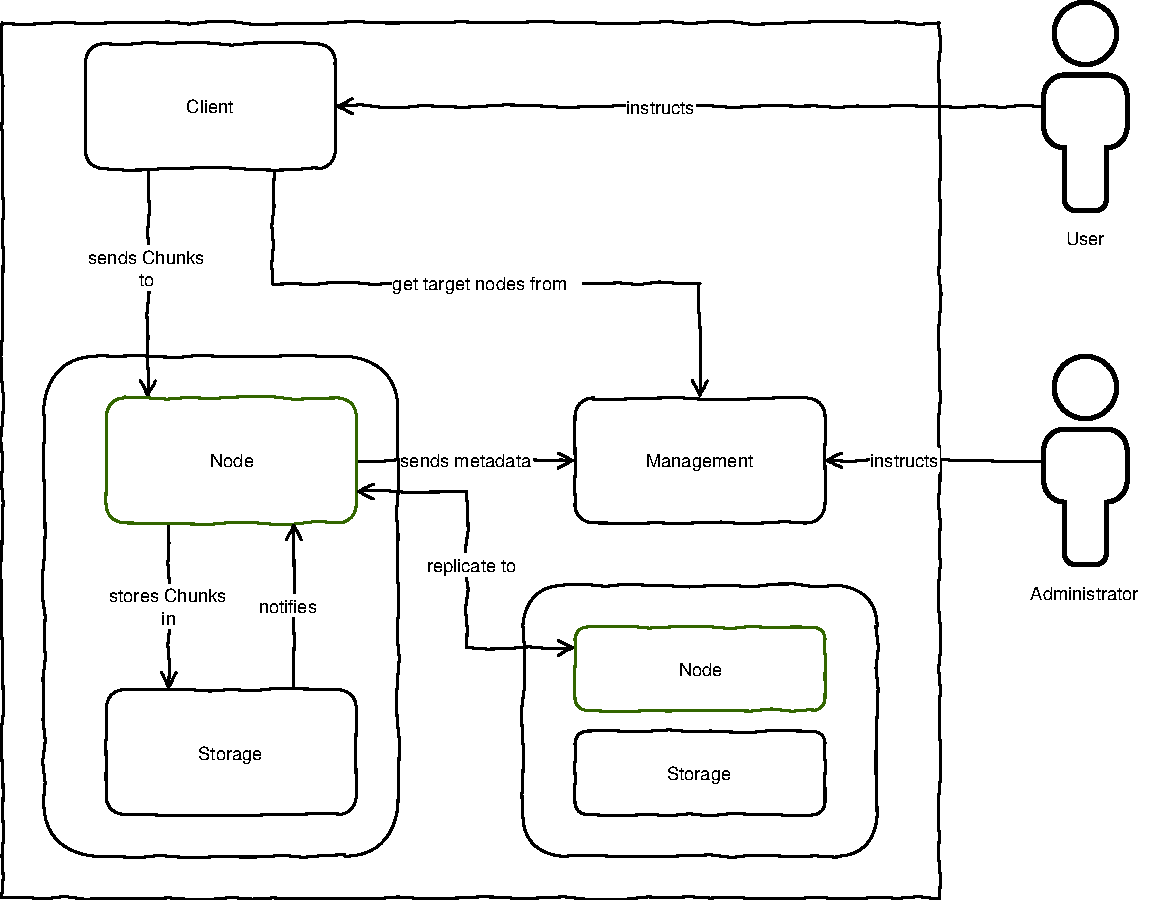
\includegraphics[width=1\linewidth]{resources/architecture_overview}
    \caption{A simplified \gls{system} overview}
    \label{fig:architecture-overview}
\end{figure}

\subsection{Actors}

\subsubsection{User}
A typical \gls{user} does not want to interact with the \gls{system} at any time. All he/she wants is to be sure that all his/her data is safely backed up.

To simplify the implementation for the study project, the \gls{user} must instruct the \gls{client} manually (create and restore backup).

\paragraph{Responsibilities}
\begin{itemize}
    \item Instruct the \gls{client} to create a Backup
    \item Instruct the \gls{client} to restore a Backup
\end{itemize}


\subsubsection{Administrator}
An \gls{administrator} wants to interact with the \gls{system} as less as possible. He/She wants to be sure that the \gls{system} runs smoothly. If something goes wrong, he/she wants to be able to fix it within a few minutes.

\paragraph{Responsibilities}
\begin{itemize}
    \item Instruct the \gls{management} to add/remove \glspl{node} from the \gls{system}
    \item Ensure that the \gls{management} runs properly (e.g. monitor it)
    \item Act if the \gls{management} notifies him/her about any anomalies
\end{itemize}

\subsection{Components}

\subsubsection{Client}
\label{sec:component-client}

\begin{figure}[h]
    \centering
    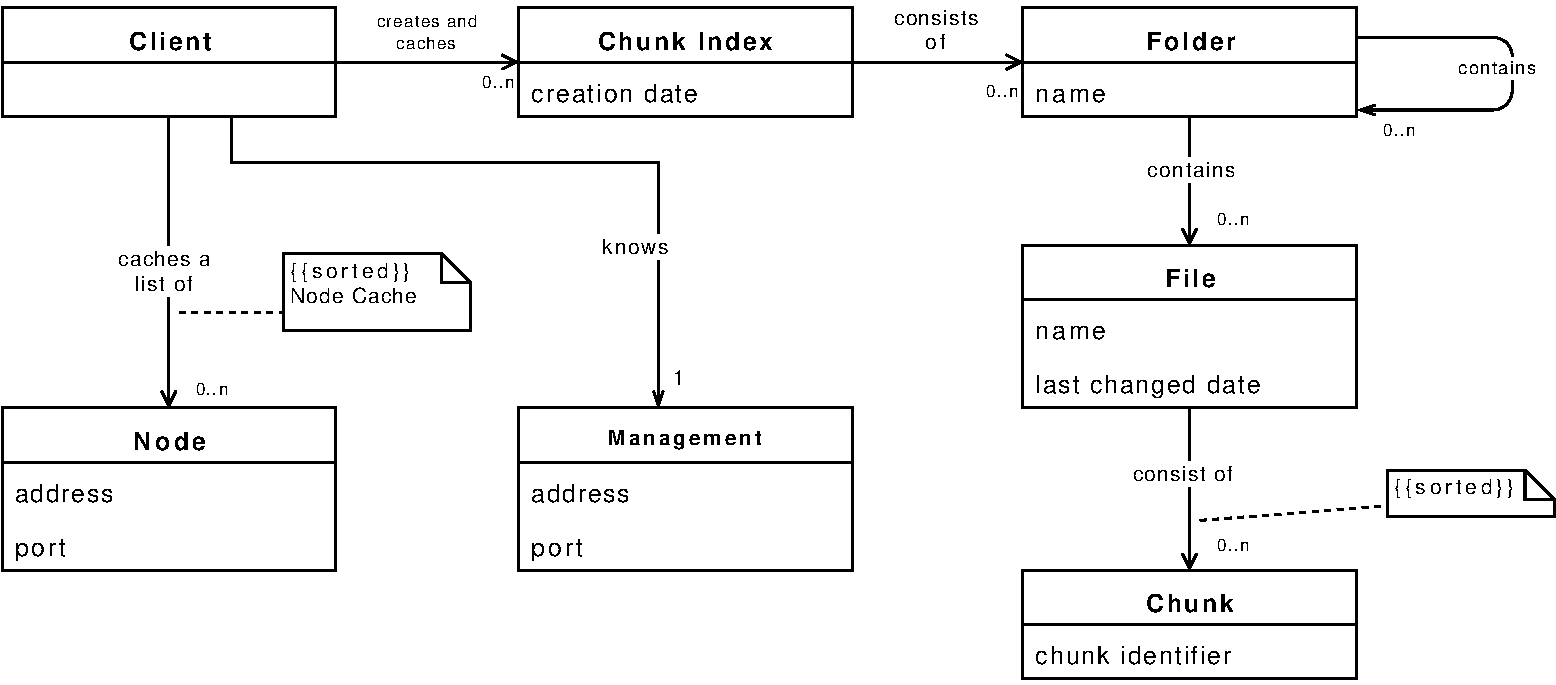
\includegraphics[width=1\linewidth]{resources/client_domain_model}
    \caption[Client Domain Model]{Domain Model illustrating the \glspl{client} perspective}
\end{figure}

\begin{itemize}
    \item The \gls{client} knows the \gls{management} by configuration.
    \item The \gls{client} queries the \gls{management} for a list of \glspl{node}, to which he can send backups or restore previous backups. He caches the results in its \gls{node-cache}.
    \item The \gls{chunk-index} hierarchically models the file system. This structure might change in the future when supporting symlinks and permissions \footnote{See e.g. \url{https://borgbackup.readthedocs.io/en/stable/internals/data-structures.html}}.
    \item The relationship between a given \gls{file} and its \glspl{chunk} is essential. The \gls{client} splits a \gls{file} into multiple \glspl{chunk} to speed up the backup of large data. During the study project, a \gls{file} consists of exactly one \gls{chunk}.
    \item A \gls{chunk} is identified by its \gls{chunk-identifier}, which can be calculated using a hash function which takes the \glspl{chunk-content}  as input.
    \item The \glspl{chunk-content} do not have be present on the \gls{client}. During backup, the \gls{client} can calculate the \glspl{chunk-content} and the corresponding \gls{chunk-identifier} from the \glspl{file} on the disk. On restore, the \gls{client} fetches the \glspl{chunk-content} from a \gls{node} and reassembles the \gls{file} based on the \gls{chunk-index}.
\end{itemize}

% TODO: Serialised Metadata = Serialised version of a given Chunk Index.

\paragraph{Responsibilities}


\begin{itemize}
    \item Keeping the \gls{node-cache} up to date
    \item Create Backups (See Scenario \ref{sec:scenario-create-backup}: \nameref{sec:scenario-create-backup})
    \begin{itemize}
        \item Building/Calculating the \gls{chunk-index}
        \item Serialize the \gls{chunk-index} into \glspl{chunk} including a \gls{root-handle}
        \item Send \glspl{chunk} to \glspl{node}
        \item Mark \glspl{chunk} as \glspl{root-handle}
    \end{itemize}
    \item Restore Backups (See Scenario \ref{sec:scenario-backup-restore}: \nameref{sec:scenario-backup-restore})
    \begin{itemize}
        \item Fetch \glspl{root-handle} from \glspl{node}
        \item Fetch \glspl{chunk} from \glspl{node}
        \item Deserialize \glspl{chunk-index}
        \item Reassemble \glspl{chunk} into \glspl{file} (not required for the study project)
        \item Let the \gls{user} choose which \glspl{file} from which \gls{chunk-index} shall be restored.
    \end{itemize}
\end{itemize}

\subsubsection{Node}

\begin{figure}[h]
    \centering
    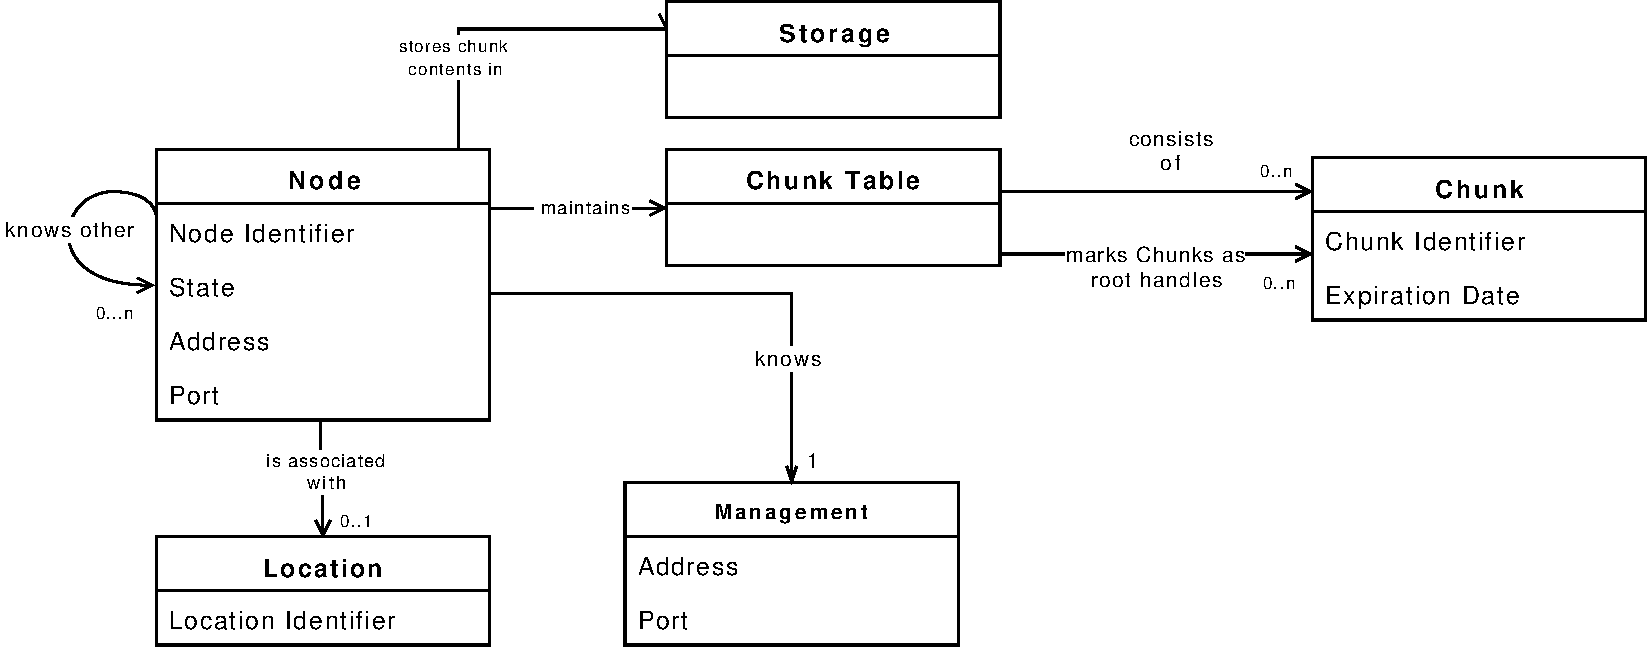
\includegraphics[width=1\linewidth]{resources/node_domain_model}
    \caption[Node Domain Model]{Domain Model illustrating the \glspl{node} perspective}
\end{figure}

\begin{itemize}
    \item A \gls{node} is identified by its unique \gls{node-identifier}. It can be addressed using a certain \emph{Address} and \emph{Port}.
    \item A \gls{node} is also associated with a \gls{location} which will be a replication criteria in the future.
    \item A \gls{node} knows the \gls{management} by configuration and exchanges data with it on a regular basis (Messages \emph{get nodes metadata} and \emph{post nodes metadata})
    \item A \gls{node} is in a given \gls{node-state} and acts differently depending on it (See Figure \ref{fig:node-states}).
    \begin{itemize}
        \item \emph{uninitialized}: The \gls{node} queries the \gls{management} for initialization and does nothing else.
        \item \emph{participating}: This is the "normal" \gls{node-state} in which a \gls{node} accepts backups, performs replication and sends requested data.
        \item \emph{unreachable}: A \gls{node} is marked as \emph{unreachable} if any other \gls{node} or the \gls{management} can not reach it. A \gls{node} never sees itself in this \gls{node-state}.
        \item  \emph{leaving soon}: The \gls{node} does not answer any requests and ensures that all its data is replicated. When it is done, it automatically switches into the \emph{left} \gls{node-state}.
        \item \emph{left}: The \gls{node} has nothing to do in this \gls{node-state} and can shut down.
    \end{itemize}
    \item A \gls{node} knows all other \glspl{node} in the \gls{system} and maintains a \gls{node-state} (see Figure~\ref{fig:node-states}) for them as well.
    \item The \glspl{chunk-content} are stored in a \gls{storage}. See \fullref{sec:component-storage} for further details.
    \item Which \glspl{chunk} are stored on the \gls{node}, their \gls{expiration-date} and the information whether a \gls{chunk} is a \gls{root-handle} is stored in the \gls{chunk-table}.
\end{itemize}

\begin{figure}[h]
    \centering
    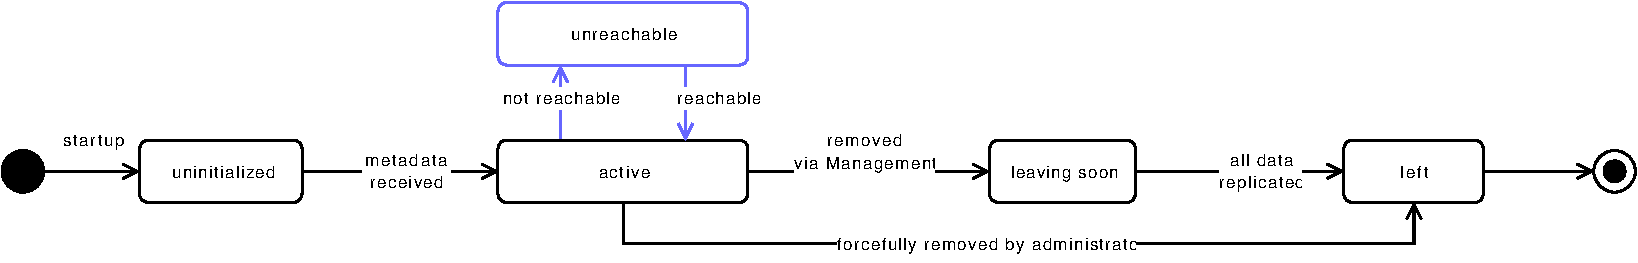
\includegraphics[width=1\linewidth]{resources/node_state}
    \caption[Node States]{A UML State Diagram describing the \glspl{node-state}}
    \label{fig:node-states}
\end{figure}

\paragraph{Responsibilities}

\begin{itemize}
    \item Send \gls{metadata} periodically (Messages \emph{get nodes metadata} and \emph{post nodes metadata}) in order to ...
    \begin{itemize}
        \item Perform initialization
        \item Learn about other \glspl{node}
        \item Start the \emph{leaving} process and notify the \gls{management} when it is completed
        \item Send \gls{metadata} to the \gls{management} so that it can perform health-checks (e.g. verify the timestamp)
    \end{itemize}
    \item Maintain the \gls{chunk-table}
    \begin{itemize}
        \item Update \glspl{expiration-date}
        \item Add new \glspl{chunk}
        \item Remove expired \glspl{chunk}
    \end{itemize}
    \item Handle possible \gls{storage} issues (see Scenario \ref{sec:scenario-storage-errors} \nameref{sec:scenario-storage-errors})
    \item Reply to \emph{get designation}  (Scenario \ref{sec:scenario-create-backup} \nameref{sec:scenario-create-backup}) , \emph{get root handles} (Scenario \ref{sec:scenario-backup-restore} \nameref{sec:scenario-backup-restore}) and \emph{get chunks} requests
    \item Replicate \glspl{chunk} (See Scenario \ref{sec:scenario-data-replication} \nameref{sec:scenario-data-replication})
    \item Handle \emph{leaving} process (see Scenario \ref{sec:scenario-node-leave-planned} \nameref{sec:scenario-node-leave-planned})
\end{itemize}

\label{sec:component-storage}
\subsubsection{Storage}

\begin{figure}[h]
    \centering
    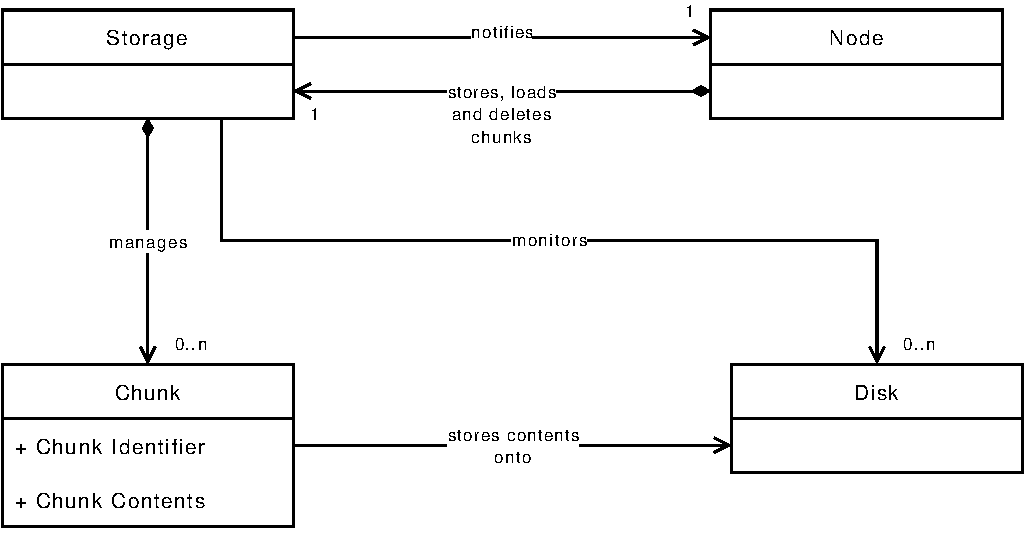
\includegraphics[width=1\linewidth]{resources/storage_domain_model}
    \caption[Storage Domain Model]{Domain Model illustrating the \gls{storage}s perspective}
\end{figure}

\begin{itemize}
    \item The main purpose of the \gls{storage} component is to persist \glspl{chunk-content}. A \gls{storage} is associated with one \gls{node} which stores, loads and deletes \glspl{chunk-content} by its \gls{chunk-identifier} on the \gls{storage}. The same \gls{node} is notified by the \gls{storage} e.g. when corrupted data is detected.
    \item A \gls{chunk} should also monitor the \glspl{medium}, on which the \glspl{chunk-content} are stored, for possible issues and report them to the \gls{node}. This feature, however, is not implemented in the study project.
    \item The \gls{storage} component is deployed on the same host as the \gls{node} that is using it.
\end{itemize}


\paragraph{Responsibilities}

\begin{itemize}
    \item Store \glspl{chunk-content}
    \item Load and return the \glspl{chunk-content} for a given \gls{chunk-identifier}
    \item Delete the \glspl{chunk-content} for a given \gls{chunk-identifier}
    \item Detect possible corruption of \glspl{chunk-content}
    \item Perform service checks on the \glspl{medium} (e.g. S.M.A.R.T tests)
    \item Notify the \gls{node} when a corruption / integrity problem occurs
\end{itemize}

\subsubsection{Management}

\begin{figure}[h]
    \centering
    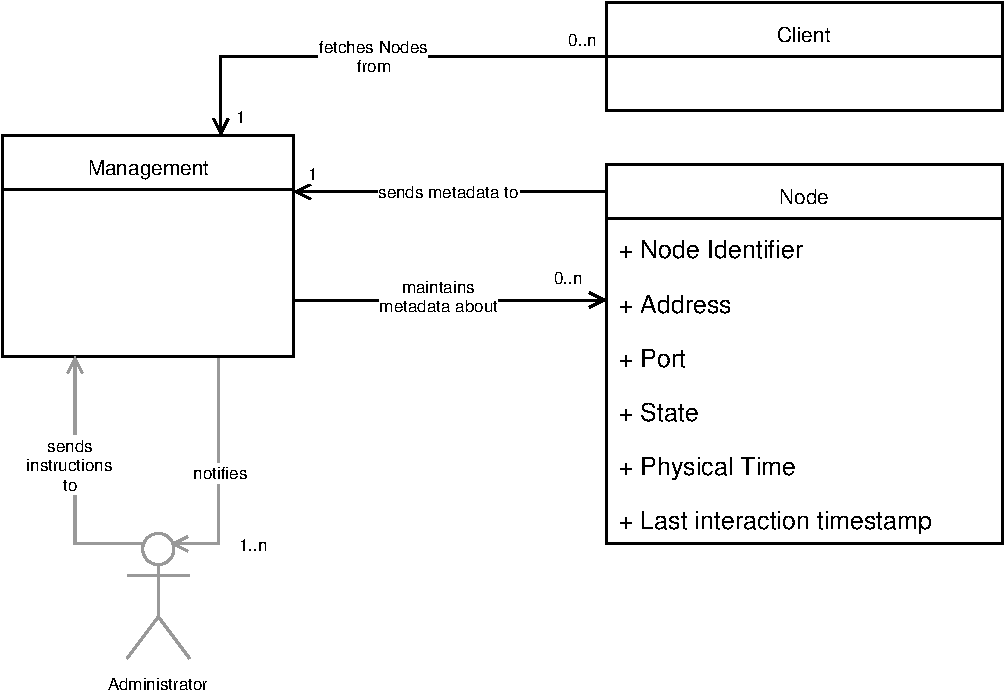
\includegraphics[width=0.75\linewidth]{resources/management_domain_model}
    \caption[Management Domain Model]{Domain Model illustrating the \gls{management}'s perspective}
\end{figure}
\begin{itemize}
    \item The \gls{administrator} is the only Actor interacting with the \gls{management}. He/She sends instructions (e.g. add new \gls{node}) and is notified by the \gls{management} about any anomalies.
    \item \glspl{client} fetch a list of all \glspl{node} from the \gls{management} (See Component \ref{sec:component-client} \nameref{sec:component-client} for further details). As for the study project, the \gls{management} does not have any information about \glspl{client}, but this might change when authentication is implemented in the future.
    \item The \gls{management} maintains \gls{metadata} for each \gls{node} in the \gls{system} and sends that information every \gls{node} when they post their \gls{metadata}.
\end{itemize}

\paragraph{Responsibilities}
\begin{itemize}
    \item Add and remove \glspl{node}
    \item Notify the \gls{administrator} e.g. if a \gls{node} leaves unexpectedly.
    \item Receive \gls{metadata} from the \glspl{node} and reply with \gls{metadata}
    \item Send list of \glspl{node} to the \glspl{client}
\end{itemize}

\subsection{Scenarios}
\label{sec:scenarios}
This section describes various scenarios of \gls{system} usage and possible failures.

In the sequence diagrams, we use the composition of the minimal integration test, detailed in Figure \ref{fig:integrationtestsmall} (Chapter \ref{integration-tests}).
The \gls{client} sends its data to \Gls{node} A only.

\subsubsection{Create Backup}\label{sec:scenario-create-backup}
The \gls{client} wants to create a backup.

\begin{figure}[h]
    \centering
    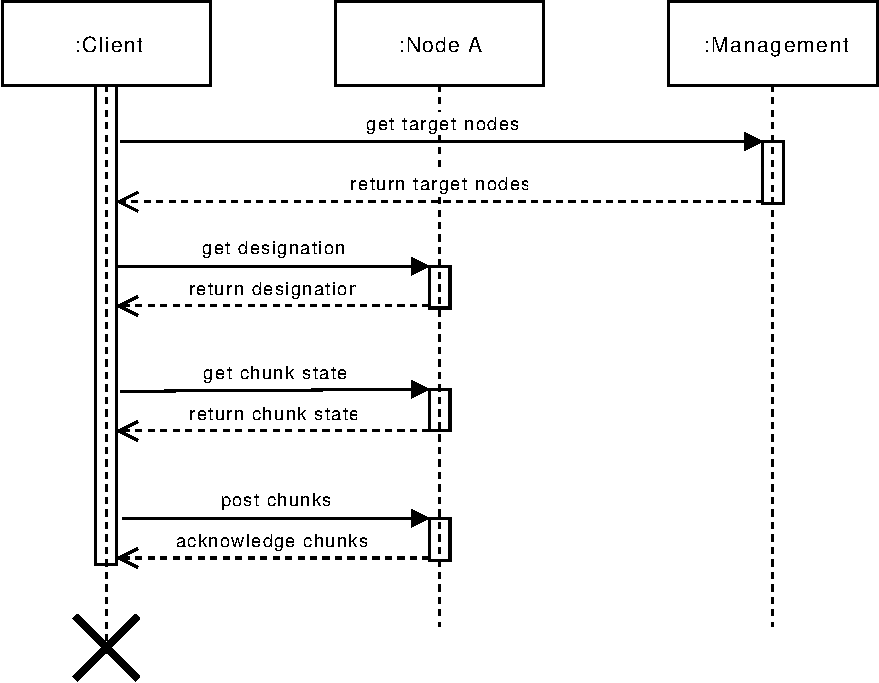
\includegraphics[width=\linewidth]{resources/create_backup}
    \caption{Create Backup Sequence Diagram}
    \label{fig:create-backup}
\end{figure}

\begin{enumerate}
    \item The \gls{client} asks the \gls{management} for a list of \glspl{node}. The \gls{management} returns a sorted list of all \glspl{node} (message: \emph{get target nodes}) (sorting might be based on specific configuration).
        \begin{itemize}
            \item If the \gls{management} is down and this is a first time backup, the \gls{client} records a message and aborts.
            \item If the \gls{management} is down, \gls{client} tries the same \glspl{node} as last time.
        \end{itemize}
    \item The \gls{client} tries to contact \glspl{node} in the presorted order.
        \begin{enumerate}
            \item The \gls{client} sends a backup request (message: \emph{get designation}).
            \item The \gls{node} acknowledges or denies the backup request (message: \emph{return designation}).
            \item If the \gls{node} acknowledges, it is declared as \gls{designated-node}.
            \item If the \gls{node} denies the backup request, the \gls{client} tries the next \gls{node}.
            \item If no \gls{node} answers the request, the \gls{client} records an error message and aborts.
       \end{enumerate}
   \item If the backup request was successful, the \gls{client} starts creating a backup.
        \begin{enumerate}
            \item The \gls{client} splits all \glspl{file} that changed since the last backup into \glspl{chunk-content} and calculate a corresponding hash, the \gls{chunk-identifier} and add it to the local \gls{chunk-index}.
            \item \Glspl{file} that have not changed since the last backup, are already be present in the \gls{chunk-index}.
            \item The \gls{client} send all \glspl{chunk-identifier} present in the \gls{chunk-index} combined with an \gls{expiration-date} to the \gls{designated-node}. (message: \emph{get chunk states})
            \item The \gls{designated-node} checks, if all \glspl{chunk-identifier} received from the \gls{client} are present in its \gls{chunk-table}.
                \begin{itemize}
                    \item If a \gls{chunk-identifier} is already present on the \gls{designated-node}, update its \gls{expiration-date} if it is further in the future.
                    \item If a \gls{chunk-identifier} is not present on the \gls{designated-node}, request it from the \gls{client} (see message response \emph{return chunk states} for further details)
                \end{itemize}
            \item The \gls{client} sends the requested \glspl{chunk-content} to the \gls{designated-node} with a \emph{post chunks} message. %TODO: Abschluss client transaktion (root handle)
                \begin{enumerate}
                    \item The \gls{designated-node} verifies and persists the \glspl{chunk-content} into its \gls{storage}. Afterwards, it acknowledges receipt to the \gls{client} (see \emph{acknowledge chunks} response message).
                                   %TODO: Client must remember, which chunks have been acknowledged. This could be done with a sliding window for QoS/memory usage?
                    \item The \gls{designated-node} replicates \gls{chunk-content} and their \gls{expiration-date} in a continuous replication process. (See scenario~\fullref{sec:scenario-data-replication})
                \end{enumerate}
            \item The \gls{client} serializes its \gls{chunk-index} into a \gls{serialised-chunk-index} and splits it into \glspl{chunk} as well. %TODO: Serialised Metadata is the chunk index plus backup metadata as linked list
            \item The \gls{client} sends the additional \glspl{chunk-content} (as \emph{post chunks} messages) to the \gls{designated-node}, in which the \gls{root-handle} is highlighted. %TODO: The root handle holds a reference to the first list chunk as well as owner etc. information.
        \end{enumerate}
\end{enumerate}

\paragraph{Special cases}
\begin{itemize}
    \item If the \gls{client} is suspended while running, it continuous with the backup process on resume. %TODO: If the expiration date is in the past, the node should refuse the chunk.
    \item If a \gls{file} is changed during the backup process, and the \glspl{chunk-content} and \glspl{chunk-identifier} cannot be calculated, the backup process must be restarted. %TODO: This may lead to starvation.
    \item If \gls{client} crashes, the backup is aborted and won't be continued if the \gls{client} is restarted.
    \item If the \gls{designated-node} goes away (disconnects/crashes/shuts down) during the backup process, the \gls{client} tries to resume the process. After a certain time (e.g. 15m), the \gls{client} gives up and restarts the backup process from the beginning.
    \item A \gls{node} must reject (i.e.\ not acknowledge) \glspl{chunk-content}, if the timestamp of the sending party (e.g. \gls{client}) is e.g.\ an hour in the future or past to prevent data loss on bad synchronized clocks.
    \item If the \gls{designated-node} runs out of storage capacity, it does reject further \glspl{chunk-content}. After a timeout, the \gls{client} restarts the backup process (with another \gls{designated-node}).
\end{itemize}

\paragraph{Possible simplifications in this study project}
\begin{description}
    \item[3a)] Do not split \glspl{file} into \glspl{chunk} but send them as is.
\end{description}

\subsubsection{Backup Restore}\label{sec:scenario-backup-restore}
The \gls{client} wants to restore specific \glspl{file}.

\begin{figure}[h]
    \centering
    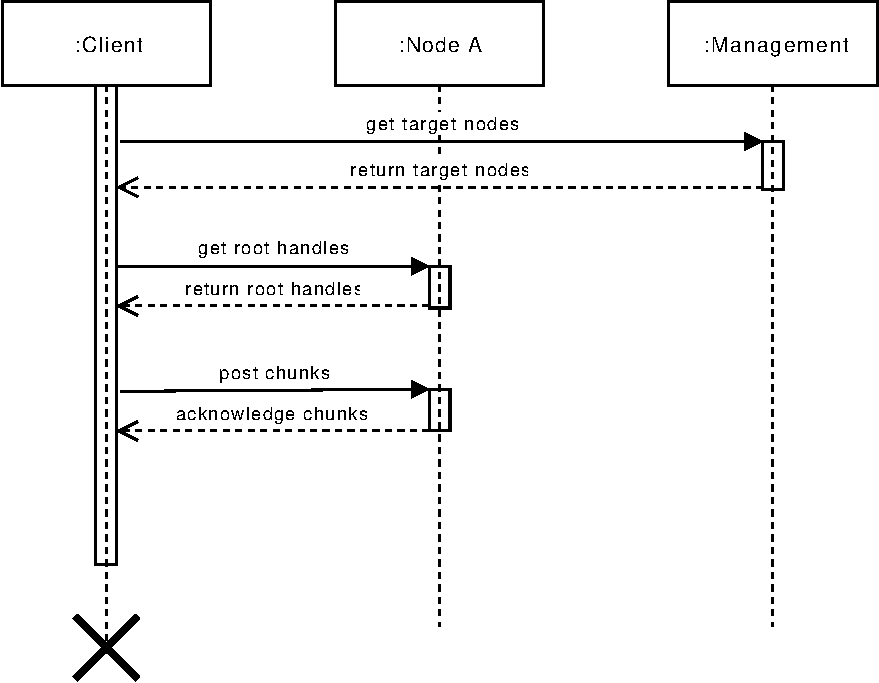
\includegraphics[width=\linewidth]{resources/backup_restore.pdf}
    \caption{Backup Restore Sequence Diagram}
    \label{fig:backup-restore}
\end{figure}

\begin{enumerate}
    \item Same as in scenario~\fullref{sec:scenario-create-backup} step 1.
    \item The \gls{client} contacts the \glspl{node} in the presorted order
        \begin{enumerate}
            \item The \gls{client} sends a \emph{get root handles} requests to a \gls{node}, the \gls{designated-node}.
            \item The \gls{designated-node} returns all \glspl{root-handle} present in the \gls{system} (see \emph{return root handles} message)
            \item If no \gls{node} answers the request,the \gls{client} records an error message and aborts.
        \end{enumerate}
    \item The \gls{client} fetches all \glspl{chunk-content} of the \glspl{serialised-chunk-index} from the \gls{designated-node} (message: \emph{get chunks}) and reassembles the \glspl{chunk-index}.
    \item The \gls{user} specifies which \glspl{file} from which \gls{chunk-index} shall be restored.
    \item The \gls{client} looks up the \glspl{chunk-identifier} in the corresponding \gls{chunk-index}.
    \item The \gls{client} requests the \glspl{chunk-content} from the \gls{designated-node}. (message: \emph{get chunks})
    \item The \gls{client} reassembles the \glspl{chunk-content} into \glspl{file}.
\end{enumerate}

\paragraph{Special cases}
\begin{itemize}
    \item If the \gls{designated-node} does not have a requested \gls{chunk-identifier} in its \gls{chunk-table}, it requests the corresponding \gls{chunk-content} recursively.
    \item If the \gls{client} crashes, the restore process must be repeated
    \item If the \gls{designated-node} is unavailable, the \gls{client} selects a new \gls{designated-node} after a certain timeout (e.g.\ 5m)
\end{itemize}

\paragraph{Possible simplifications in this study project}
\begin{description}
    \item[-] The \gls{client} must request a \gls{node} that has the data already available (possibly the \gls{designated-node}, where the backup was created).
\end{description}


\subsubsection{Node Joining}\label{sec:scenario-node-join}
A \gls{new-node} joins the \gls{system}.

\begin{figure}[h]
    \centering
    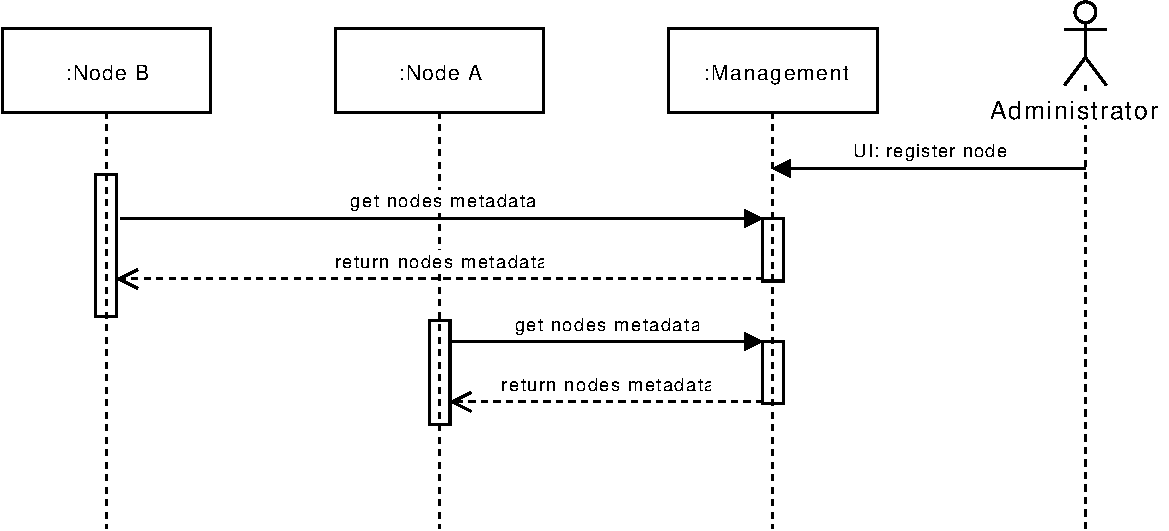
\includegraphics[width=\linewidth]{resources/node_joining.pdf}
    \caption{Node Joining Sequence Diagram}
    \label{fig:node-joining}
\end{figure}

This scenario is described as it is implemented in the study project. It might be subject to further evaluation in the future.

\begin{enumerate}
    \item The \gls{new-node} is registered by an \gls{administrator} in the \gls{management} using its \gls{node-identifier}. A \gls{location} must also be assigned to the \gls{node}. %TODO: Data
    \item The \gls{new-node} queries \gls{metadata} from the \gls{management} (message: \emph{get nodes metadata}) on startup.
    \item The \gls{new-node} configures itself based on its \gls{node-identifier} and received \gls{metadata} from \gls{management}.
        \begin{itemize}
            \item If the \gls{management} has no information available (yet) or is unavailable, the \gls{new-node} retries after a certain timeout (e.g.\ 5min).
        \end{itemize}
    \item Other \glspl{node} learn about the \gls{new-node} through periodical \gls{metadata} queries (message: \emph{post nodes metadata})
        \begin{enumerate}
            \item If the \gls{new-node} contacts an existing \gls{node}, before the existing \gls{node} updates its \gls{metadata}, the existing \gls{node} should query the \gls{management} (message: \emph{get nodes metadata})
            \item If the \gls{management} is unavailable, the \gls{new-node} ignores all communication attempts.
        \end{enumerate}
\end{enumerate}

\subsubsection{Node Leaving Planned}\label{sec:scenario-node-leave-planned}
A \gls{node} leaves the \gls{system} planned (refered as \gls{leaving-node}).

\begin{figure}[h]
    \centering
    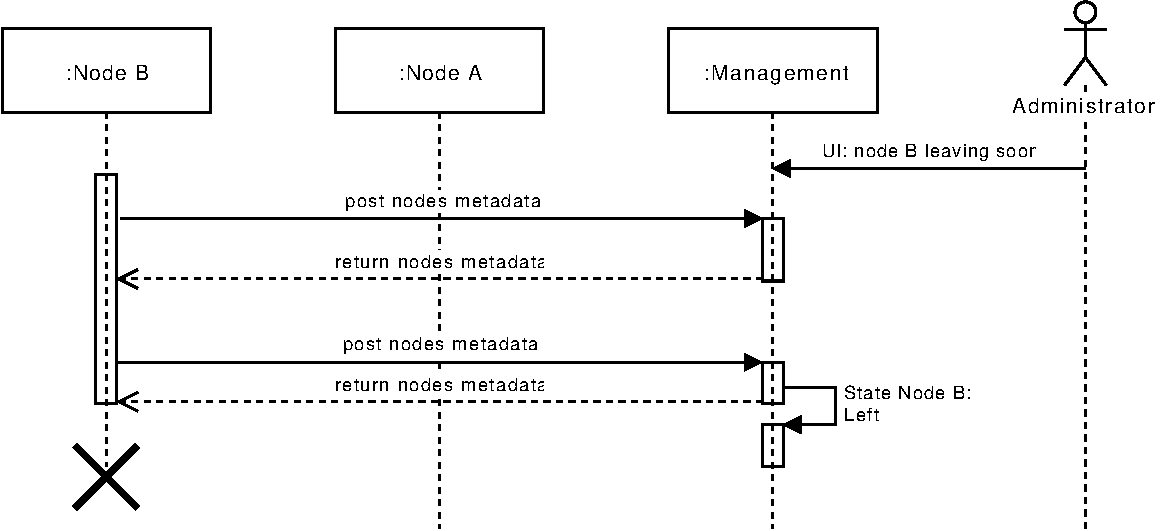
\includegraphics[width=\linewidth]{resources/node_leaving_planned.pdf}
    \caption{Node Leaving Planned Sequence Diagram}
    \label{fig:node-leave-planned}
\end{figure}

This scenario is described as it is implemented in the study project. It might be subject to further evaluation in the future.

\begin{enumerate}
    \item The \gls{leaving-node} is marked as \emph{leaving soon} by the \gls{administrator} in the \gls{management}.
    \item As soon as the \gls{leaving-node} realises that it is in \gls{node-state} \emph{leaving soon} (using \emph{post nodes metadata}), it ignores messages from other \glspl{node}, rejects any new backups and starts replicating its \glspl{chunk-content} to another \gls{node}.
    \item As soon as all \glspl{chunk-content} are replicated onto other \glspl{node}, the \gls{leaving-node} changes its \gls{node-state} to \emph{left} and informs the \gls{management} (message: \emph{post nodes metadata}).
\end{enumerate}

\subsubsection{Node Leaving Unplanned}\label{sec:scenario-node-leave-unplanned}
A \gls{node} leaves the \gls{system} unexpectedly.

\begin{figure}[h]
    \centering
    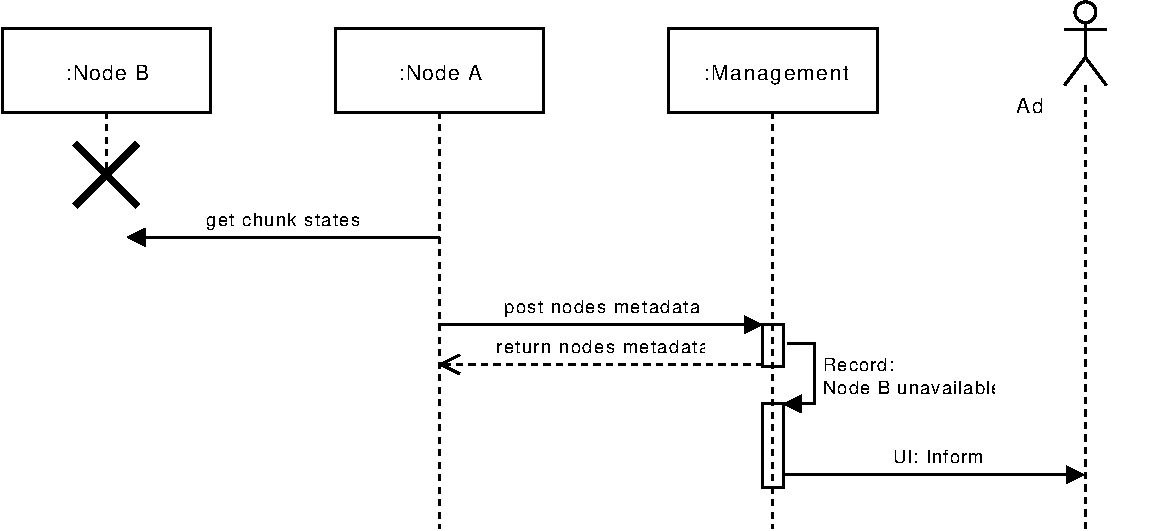
\includegraphics[width=\linewidth]{resources/node_leaving_unplanned.pdf}
    \caption{Node Leaving Unplanned Sequence Diagram}
    \label{fig:node-leave-unplanned}
\end{figure}

This scenario is described as it is implemented in the study project. It might be subject to further evaluation in the future.

\begin{enumerate}
    \item If a \gls{node} is not responding (which means, no other \gls{node} nor the \gls{management} can reach it), the \gls{management} records the unavailability and informs the \gls{administrator}.
    %Replikationsmechanismus; management knows, that on reason of intervall the node is away
\end{enumerate}

\begin{itemize}
    \item If the \gls{node} returns, it carries on as if nothing happend.
    \item If the \gls{node} does not return, the \gls{administrator} marks the \gls{node} as \emph{left}, which is propagated to all \glspl{node} via the \emph{post nodes metadata} message.
        \begin{itemize}
            \item \glspl{chunk-content}, which were not previously replicated from the \gls{node} are lost.
        \end{itemize}
\end{itemize}

\subsubsection{Data Replication}\label{sec:scenario-data-replication}
The network distributes \glspl{chunk}.

\begin{figure}[h]
    \centering
    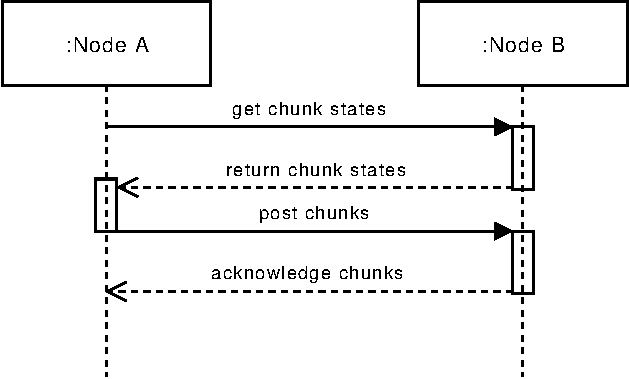
\includegraphics[width=0.6\linewidth]{resources/data_replication.pdf}
    \caption{Data Replication Sequence Diagram}
    \label{fig:data-replication}
\end{figure}

This scenario is described as it is implemented in the study project. It might be subject to further evaluation in the future.

\begin{enumerate}
    \item The \gls{sending-node} picks $n$ random entries from its \gls{chunk-table}. In the future, these entries might be selected based on heuristics.
    \item The \gls{sending-node} picks one random \gls{designated-node} from its \gls{metadata}. In the future, the \gls{designated-node} might be selected based on heuristics.
    \item The \gls{sending-node} sends the \glspl{chunk-identifier} of the chosen entries to the \gls{designated-node} with a \emph{get chunk states} message.
    \item The \gls{designated-node} checks, if all \glspl{chunk-identifier} received from the \gls{sending-node} are present in its \gls{chunk-table}.
        \begin{itemize}
            \item If a \gls{chunk-identifier} is already present, update its \gls{expiration-date} if it is further in the future.
            \item If a \gls{chunk-identifier} is not present, request the corresponding \gls{chunk-content} from the \gls{sending-node} (see message \emph{return chunk states} for further details).
        \end{itemize}
    \item The \gls{sending-node} sends the requested \glspl{chunk-content} to the \gls{designated-node} with a \emph{post chunks} message.
        \begin{itemize}
            \item The \gls{designated-node} verifies and persists the \glspl{chunk-content} into its \gls{storage}. Afterwards, it acknowledges receipt to the \gls{sending-node} (see \emph{acknowledge chunks} response message).
        \end{itemize}
\end{enumerate}

\subsubsection{Data has Expired Lifetime}\label{sec:scenario-data-expiration}
A \gls{node} wants to delete \glspl{chunk} with a past \gls{expiration-date}.

This scenario is described as it is implemented in the study project. It might be subject to further evaluation in the future.

\begin{itemize}
    \item The \gls{management} monitors the \glspl{node} physical timestamp and records any deviation from the \gls{management} time larger than 1h.
    \item Therefore, a first prototype, the \gls{node} may just delete \glspl{chunk} after the specified \gls{expiration-date} without further checks.
        \begin{itemize}
            \item We build on the assumption, that the \glspl{node} have different upstream timeservers, so that a general time shift is unlikely.
            \item In case a single \gls{node}s time is in the past, and runs out of storage capacity, it might lead to a redundancy loss.
            \item If a single \gls{node}s time is in the future, the redundancy is reduced by one.
        \end{itemize}
\end{itemize}

In the future, it is advisable to implement a consent protocol to reduce the likelihood of data loss.

\subsubsection{Data Storage has Errors}\label{sec:scenario-storage-errors}
The \gls{storage} component notifies its \gls{node} that a \gls{chunk} stored in it is corrupt.

This scenario is described as it is implemented in the study project. It might be subject to further evaluation in the future.

\begin{enumerate}
    \item The \gls{storage} informs the \gls{node} of a corrupt \gls{chunk} using its \gls{chunk-identifier}
    \item The \gls{node} removes the \gls{chunk-identifier} from the \gls{chunk-table}
        \begin{itemize}
            \item The \gls{chunk} will be replicated eventually.
        \end{itemize}
    \item Inform \gls{management} when sending the next \emph{post nodes metadata} message.
\end{enumerate}

\subsubsection{Management Problems}\label{sec:scenario-management-problems}
\begin{itemize}
    \item The case, that the \gls{management} has outdated \gls{metadata} out of a data loss, will be ignored during this study project. A mechanism solving this problem, would probably be subject to significant changes in further development e.g.\ when implementing limited redundancy levels. %TODO: Counter in config in the future
\end{itemize}

\subsubsection{Network Availability Problems}\label{sec:scenario-network-errors}
\paragraph{Behaviour in case a node can reach only some nodes directly}
The still available \glspl{node} should try to satisfy redundancy needs as good as possible.
If a \gls{node} cannot reach other \glspl{node}, it notifies the \gls{management} with the next \emph{post nodes metadata}

\paragraph{Behaviour in case the network gets partitioned}
(, and the \glspl{node} in each partition can only reach each other and not the other ones.)

See first case in scenario~\fullref{sec:scenario-network-errors}

\paragraph{Behaviour in case nodes have different states of management information}
The redundancy is temporary reduced to the \glspl{node} which the group of old \glspl{node} know, but will eventually be resolved as \glspl{node} fetch \gls{metadata}.


\subsection{Messages}\label{sec:messages}
\Glspl{message} denote the communication units between application components. A \gls{message} is wrapped by an \gls{envelope}.

\subsubsection{Envelopes}
An \gls{envelope} is a wrapper for a \gls{message}, which provides standardised attributes.

\begin{table}[h]
    \begin{tabu}{>{\ttfamily}l X}
        timestamp\_now
            & The current UTC time of the local clock as a unix timestamp.  \\
        message\_type
            & A string representation of the type of the message, as described in chapter \fullref{sec:messages}. \\
        message
            & The actual payload of the specified \texttt{message\_type}
    \end{tabu}
    \caption[\Gls{envelope} Structure]{Structure of an \gls{envelope}.}
    \label{tab:envelope}
\end{table}

\subsubsection{get target nodes}
A \gls{client} requests a list of \glspl{node} from the management, with the indent to make backups on. The client expects a \emph{return target nodes} \gls{message} in return.

The \gls{message} is empty.

\subsubsection{return target nodes}
The \gls{node} responds to the \glspl{client} request \emph{get target nodes}.

\begin{table}[h]
    \begin{tabu}{>{\ttfamily}l X}
        target\_nodes
            & A list of possible \emph{target nodes} as described in Table \ref{tab:message-return-target-nodes-field-target-nodes}. The list is sorted in descending order by preference, defined by the \gls{management}.
    \end{tabu}
    \caption[\emph{return target nodes} Structure]{Structure of a \emph{return target nodes} \Gls{message}.}
    \label{tab:message-return-target-nodes}
\end{table}

\begin{table}[h]
    \begin{tabu}{>{\ttfamily}l X}
        hostname
            & Hostname of the \gls{node}. \\
        ip\_address
            &  IP-Address of the \gls{node}. \\
        port\_number
            &  Port-Number of the \gls{node}. \\
    \end{tabu}
    \caption[Field \texttt{target\_nodes} Structure]{Structure of Field \texttt{target\_nodes} as Used in the \emph{return target nodes} \Gls{message}.}
    \label{tab:message-return-target-nodes-field-target-nodes}
\end{table}

\subsubsection{get designation}
GET: estimate size; identification; how long data stored
\subsubsection{return designation}
 RETURN: agree; not agree (reason)

\subsubsection{get chunk states}
\subsubsection{return chunk states}
RETURN: chunk identifiers; keep date; stored (boolean); chunk handle state(boolean)

\subsubsection{post chunks}
POST: chunk identifier; chunk data; how long data stored; root handle state
\subsubsection{acknowledge chunks}
ACK: chunk identifier; stored(boolean)

\subsubsection{get chunks}
GET: chunk identifier
\subsubsection{return chunks}
RETURN: chunk identifier, chunk data; root handle state

\subsubsection{get root handles}
GET: userid
\subsubsection{return root handles}
RETURN: chunk identifier; chunk data

\subsubsection{get nodes metadata}
\subsubsection{post nodes metadata}
POST: current local node metadata(identifier; state; redundancy status; free storage; capacity); current "neightbour" status(identifier;state)
\subsubsection{return nodes metadata}
RETURN list of (node name; node ip; node state; node free storage)


% !TeX spellcheck = en_GB
\section{Fundamental Design Decisions} % TODO: better name?

We used the morphological box technique to explore different possible solutions.

The chosen option should be as simple as possible for the prototype developed in the study project but extensible for further adaption.

The following paragraphs reason the selected entry in each dimension.

\paragraph{Redundancy} 
We originally planned to support \emph{client m-replication}. This, however, is a complex mechanism that requires sophisticated algorithms to work correctly and efficiently. We chose the system \emph{n-replication} option because it is simple to implement in a prototype. Changing this option in the future is hard because it requires fundamental changes in the replication process and the communication protocols.

\paragraph{Storage unit}
The idea of \emph{chunks} come from Borg Backup. Files are partitioned into chunks using a rolling hash which allows deduplication as well as space efficient backups for large files \cite{borg-data-structures}. These are desired properties in a backup system to minimise network and disk usage.

\emph{Encrypting chunks} means that deduplication of the same file coming from different users is not possible anymore but is a necessity for privacy. Encryption is not trivial and requires a user concept that is out of scope of the prototype developed in the study project.
We chose the \emph{plain filesystem} option for the study project to simplify the client implementation. Supporting \emph{encrypted chunks} in the future is possible by just modifying the client.

\paragraph{Role of the management}
The \emph{one in charge} option is the most straightforward option to implement but conflicts with many intentions of the administrator (See \fullref{sec:adminstrator-intention}). We also intended to avoid a single point of failure. We chose the option \emph{autonomous replication} because it guarantees that replication is always ensured and keeps communication relatively simple.

\paragraph{Storage backend}
Using the file system is the simplest possible solution for the study project and therefore selected option. Adding support for other backends in the future is still possible since the storage component is an isolated part of the architecture (See \fullref{sec:component-storage})

\paragraph{Removal of old backups}
We propose to use a fixed \emph{physical time} that must be specified on backup creation. After expiration, the backup data may be removed by a garbage collector. This may be extended to allow only mutual garbage removal in the future.

A significant problem that \emph{physical time} addresses is the safety of backup data in case a user computer is infected with malware. An illicit application might command the removal of backups, or create new backups to initiate a garbage collection process to free storage capacity.

Nevertheless, the use of \emph{physical time} has the downside of possible data loss due to wrong system times. To lessen this risk, the system should use multiple distinct upstream time-servers. This is given with a high probability, as the proposed redundancy model motivates users to expand the system across multiple physical locations. Furthermore, the client, nodes and management should verify a reasonable accurate time when communicating mutually.

\paragraph{Programming language / ecosystem}
A complete language evaluation can be found in \fullref{sec:language-evaluation}.


\begin{sidewaystable}
	\centering
	\caption[Morphological Box]{Morphological Box}
	\label{tbl:morphological-box}
    \begin{tabu}{X | X X X X}
		\hline
          \textbf{Redundancy}
          & No redundancy
          & Client m-replication: The client defines a custom degree of redundancy (from 1 to the number of nodes).
          & System m-replication: The administrator defines the degree of redundancy for the whole system (from 1 to the number of nodes).
          & \textbf{System n-replication}: The degree of redundancy for the whole system is equal to the amount of nodes in the system.
          \\ \hline

          \textbf{Storage unit}
          & \textbf{Plain files}
          & Encrypted files
          & Chunks: Cut files into multiple parts and store these individually.
          & Encrypted chunks: Same as chunks, but every chunk is individually encrypted.
          \\ \hline


          \textbf{Role of the management}
          & One in charge: The management knows and controls everything (e.g. the location of every file/chunk).
          & Configuration only: The management must be up for administrative tasks only. The nodes are mostly autonomous.
          & \textbf{Autonomous replication}: The management must be available for most of the tasks but replication also works if the management is down.
          & No management: Every node is completely autonomous.
          \\ \hline


          \textbf{Storage backend}
          & \textbf{Plain filesystem}: Just store all files/chunks as files in one directory with a unique identifier.
          & Database: Use an existing database solution (e.g. Git, Redis, RocksDB).
          & Cloud Storage: A proxy to a cloud storage provider (e.g. Amazon S3).
          & Custom: An optimized version of the plain file system option with optimised indexing and compression.
          \\ \hline


          \textbf{Removal of old backups}
          & \textbf{Physical time}: Data is removed on a specified physical time.
          & User command: The user commands removal of data.
          & Free storage: Data is removed, as soon as capacity issues occur.
          & Physical time with mutual agreement: All nodes must agree before data is removed.
          \\ \hline


          \textbf{Programming language / ecosystem}
          & \textbf{Rust}
          & Go
          & Erlang
          & 
          \\ \hline
	\end{tabu}
\end{sidewaystable}

\subsection{Hash Collisions}
To achieve deduplication and space-efficient backups for large files, as discussed above, a file/chunk identifier must be derived from the actual file/chunk contents. 
A common mechanism used to derive identifiers from binary data are cryptographic hash functions. Most cryptographic hash functions produce a message digest having a fixed size (e.g. SHA256 produces a 256-bit digest) for a message with an arbitrary length, which can theoretically lead to collisions.
Perfect hash functions do not have this property because their input message size is fixed and equal to the size of the resulting message digest. A perfect hash function is not practical in our case due to the large message digests.
With cryptographic hash function, collisions are possible but unlikely. Assuming that the applied function does produce equally distributed results, the probability can be calculated based on the birthday problem\cite{birthday-attack} as follows, where $p$ is the number of chunks in the system and $n$ the size of the message digests:

\[
P(p, n) = \frac{p^2}{2^{n+1}}
\]

Assuming we have $p=30^{21}$ files/chunks the system (which is equivalent to two billion years of music assuning each chunk has a size of one byte\cite{seagate-zetabyte}) and using the SHA-256 algorithm, the probability of collisions is about $4.72 \cdot 10^{-16}$, which is almost 0 and can almost be neglected.

If, however, a collision happens after all, for example, if the used cryptographic hash function is flawed or the unlikely event occurs, it results in data loss.

As for the study project, we use the SHA-256 algorithm and neglect the risk of hash collisions due to its low probability. Nonetheless, we prepare all protocols and components to use an interchangeable mechanism for the calculation and transmission of the identifiers.

% !TeX spellcheck = en_GB
\section{Language Evaluation}

Based on the Requirements described in Appendix \ref{requirements}, we compared three languages/technologies.

We heard of \textbf{Rust} as being a modern language as an alternative to the traditional ''low-level'' languages C and C++.

\textbf{Erlang} was the second candidate of which we heard that it is well suited for distributed, fault-tolerant systems. It is also a functional programming language, with which we both do not have much experience but share an interest in it.

\textbf{Go} came up when researching for distributed systems in Rust. Friends, as well as various blog posts, suggested Go is established in the field of distributed systems, has a diverse eco-system and is therefore well suited for the job.

We grouped the criterions for our comparison into three groups: Client (See Table \ref{language-comparison-client}), Distributed System  (See Table \ref{language-comparison-ds}) and Eco System  (See Table \ref{language-comparison-eco-system}). The assessment is not entirely objective and based on a brief research as well as personal impressions.

\begin{table}[h]
	\centering
	\caption{Language and Ecosystem Comparison for the Client}
	\label{language-comparison-client}
	\begin{tabu}{X|X X X}
		\hline
		\diagbox[width=9em,height=2.5em]{Criteria}{Language}
		& Rust
		& Erlag
		& Go
		\\ \hline

		platform independent
		& Yes, LLVM Backend \cite{rust-blog-introducing-mir}
		& Yes \cite{erlang-faq-implementations}
		& Yes \cite{go-github-minimum-requirements}
		\\
		
		allow an easy installation (no runtime required or bundle it)
		& Runtime included, compiles to machine code via LLVM \cite{rust-blog-introducing-mir}
		& No \cite{erlang-packaging}
		& Creation of statically-linked binaries by default \cite{golang-org-faq}
		\\
		
		
		bindings to a reasonable (platform independent) UI-Framework
		& No, lots of tools are in in alpha stage. See \url{https://github.com/rust-unofficial/awesome-rust\#gui}
		& No \cite{stackoverflow-erlang-guis}
		& Yes, See \url{https://github.com/avelino/awesome-go\#gui}
		\\
	\end{tabu}
\end{table}

\begin{table}[h]
	\centering
	\caption{Language and Ecosystem Comparison for the Distributed System}
	\label{language-comparison-ds}
	\begin{tabu}{X|X X X}
		\hline
		\diagbox[width=9em,height=2.5em]{Criteria}{Language}
		& Rust
		& Erlag
		& Go
		\\ \hline

		run on lightweight (cost effective) platforms such as a raspberry pi.
		& Yes, through LLVM \cite{rust-blog-introducing-mir}
		& Yes \cite{erlang-faq-implementations}. Different Semantics: Run in a cluster
		& Yes \cite{go-github-minimum-requirements}
		\\
		
		fast / efficient
		& Yes, "zero cost abstraction" and "minimal runtime" \cite{rustlang-org}, LLVM optimizer \cite{rust-blog-introducing-mir}
		& Yes, using the Actor Model \cite{hebert_learn_you_some_erlang}
		& Yes, using the Goroutines \cite{doxsey_introduction_2012}
		\\
		
		safe concurrency for networking and calculation of checksums
		& Yes, using borrow and move semantics \cite{rust-book-concurrency}
		& Yes, using the Actor Model \cite{hebert_learn_you_some_erlang}
        & Yes, using the Goroutines \cite{doxsey_introduction_2012}
		\\
		
		Use existing libraries (e.g. for reading disk health status)
		& Yes, using FFI \cite{rust-book-concurrency}
		& Yes, using NIF \cite{erlang-org-nif}
		& Yes, using cgo \cite{golang-org-cgo}
		\\
		
		provide a stable and fast network stack
		& Yes, in the standard library as well as frameworks such as Tokio \cite{tokio-rs}
		& Yes, in the standard library \cite{erlang-org}
		& Yes, in the standard library \cite{golang-org}
		\\
		
	\end{tabu}
\end{table}

\begin{table}[h]
	\centering
	\caption{Language and Ecosystem Comparison for the Eco System}
	\label{language-comparison-eco-system}
	\begin{tabu}{X|X X X}
		\hline
		\diagbox[width=9em,height=2.5em]{Criteria}{Language}
		& Rust
		& Erlag
		& Go
		\\ \hline

		Web frameworks (for the management)
		& Yes, e.g. \url{https://gotham.rs/}
		& Yes, e.g. \url{http://chicagoboss.org/}
		& Yes, e.g. \url{https://beego.me/}
		\\
		
		Stability
		& "stability without stagnation" \cite{rust-blog-stability}
		& Yes, first release in 1986 \cite{erlang-org}
		& Stabile, release every 6 months \cite{go-github-release-cycle}
		\\
		
		stable libraries for common tasks
		& More than 11'000 on \url{https://crates.io/}
		& More than 5'000 Packages available on \url{https://hex.pm/}
		& More than 756'00 golang Repositories indexed on \url{http://go-search.org/} (includes all GitHub forks as well)
		\\
		
		productive tooling
		& Cargo, IDE-Support (VS-Code, IntelliJ Rust etc)
		& rebar3, IDE-Support (erlide, IntelliJ Erlang etc)
		& dep not yet that established but dependency management via `go get` IDE-Support (VS-Code, Goland etc)
		\\
		
		good testing frameworks (unit and integration tests)
		& Included (cargo test) as well as other testing frameworks
		& Included (EUnit)
		& Included (testing) as well as other testing frameworks
		\\
		
		good and up to date documentation
		& Yes, Rust Book, Good Documentation of the standard library, other Literature
		& Yes, User Guide, Good Documentation of the standard library, other Literature
		& Yes, Good Documentation of the standard library, other Literature
		\\
		
		active community to get support
		& Yes, via IRC, Forum and more. See \url{https://www.rust-lang.org/en-US/community.html}
		& Yes via IRC/Slack, Forum and more. See \url{http://www.erlang.org/community}
		& Yes via IRC/Slack, Forum and more. See \url{http://www.erlang.org/community}
		\\
		
		Support bug-free coding (e.g. good type system, memory safety, linting or good compiler)
		& Yes, Linter, Borrow-Checker. No good metrics / coverage libraries yet.
		& Yes, Linter, Coverage Tools etc.
		& Yes, Linter, Coverage Tools etc.
	\end{tabu}
\end{table}

\subsection{Decision}
We decided to use Rust. Although it is still a rather young language, it has a very enthusiastic and welcoming community, stable releases and an excellent documentation.

The main reason we settled for Rust was its type system as well as the concept of Ownership and Borrowing, which enables so many of Rusts features and permits us to do safe concurrency. Also, Rust has two excellent networking libraries.

The most significant downside to Rust for us is the limited amount of high-quality libraries.

We ruled out Erlang because of three reasons. Firstly, since we do not have any experience with functional programming languages, we expect a much steeper learning curve and therefore slower progress. Secondly, we think that we do not need most of Erlangs key features such as Hot Swapping and strong process isolation. At last, Erlang requires to be run in the Erlang VM, which makes deployment more difficult than in Rust or Go.

In comparison to Rust, Go lacks various features. For example, the lack of generics, having a garbage collector and pointers lead to more memory consumption and higher parallelisation risks. An advantage of Go is a slightly more established ecosystem.
% !TeX spellcheck = en_GB

\section{Testing}
\label{testing}

In the following chapters we illustrate, how we test our prototype and architecture.

\subsection{Unit Tests}\label{unit-tests}
As we use test driven development (TDD) to develop the prototype, we make heavy use of unit tests. Our Definition of Done\cite{project-plan} states that \emph{reasonable unit and integration tests [must] exist and pass.}

Therefore, these tests are executed on every build run of our continuous integration, that is on every repository push and pull request.


\subsection{Integration Tests}\label{integration-tests}
Our integration tests are split into two main environments: A minimal one as defined in figure \ref{fig:integrationtestsmall} and a medium network, as defined in figure \ref{fig:integrationtestmedium}.

\begin{figure}
	\centering
	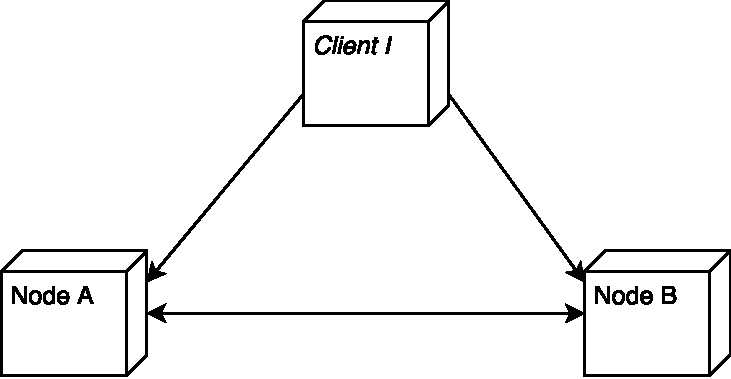
\includegraphics[width=0.5\linewidth]{resources/integration_test_small}
	\caption[Minimal integration test]{Minimal integration test with one client and two nodes.}
	\label{fig:integrationtestsmall}
\end{figure}

\begin{figure}
	\centering
	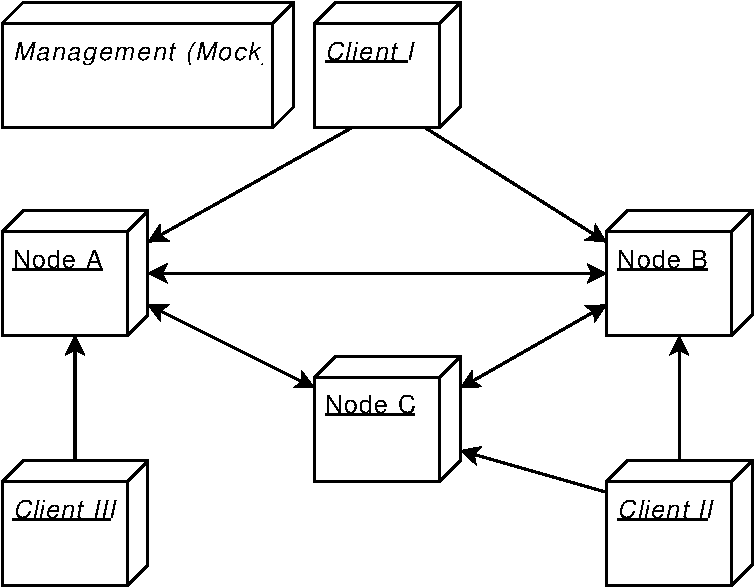
\includegraphics[width=0.5\linewidth]{resources/integration_test_medium}
	\caption[Medium integration test]{Medium integration test with three clients and three nodes.}
	\label{fig:integrationtestmedium}
\end{figure}

These two, rather small nework styles will probably be the most commonly used deployments, yet cover most of the possible problems that may occur.

On these two networks, the implemented scenarios as defined in appendix \ref{scenarios} are tested (if applicable).

The integration tests are to be run on every tagged release (i.e. at least once every sprint).

\subsubsection{Implementation}

To bootstrap the infrastructure we utilise Docker Compose, a tool for defining and running multi-container Docker applications\cite{docker-compose}. The node application, as well as the client and a managment mockup are run in separate containers, connected over a virtual network.

\subsection{Architecture tests}

Architectural tests are special, manually run tests to verify the scalability of our software architecture.

\subsubsection{Size scalability}
As per our requirements in appendix \ref{requirements}, the architecture should scale up to 100 nodes. To test this scenario, we use the same underlying techniques as in our integration tests (see chapter \ref{integration-tests}), but scale the infrastructure up to the required limits.

\subsubsection{Network data capacity}
Our requirements (appendix \ref{requirements}) also state, that a node must be able to handle up to e.g. 2TB of data. To test this requirement, we create large amounts of random data that has to be stored. This is a realistic requirement, as e.g. a compressed image, audio and movie collection might reach such sizes in practice.



%----------------------------------------------------------------------------------------
%	DECLARATION PAGE
%----------------------------------------------------------------------------------------

\begin{declaration}
\addchaptertocentry{\authorshipname} % Add the declaration to the table of contents
\noindent We, \authorname, declare that this thesis and the work presented in it are our own, original work.  All the sources we consulted and cited are clearly attributed. We have acknowledged all main sources of help. \\

\noindent Fabian Hauser\\[2em]
\rule[0.5em]{25em}{0.5pt}\\ % This prints a line for the signature
\noindent Raphael Zimmermann\\[2em]
\rule[0.5em]{25em}{0.5pt}\\ % This prints a line for the signature 
\noindent Rapperswil, \today
\end{declaration}

\cleardoublepage


%----------------------------------------------------------------------------------------

\end{document}  
